% !TeX spellcheck = de_DE
\documentclass[12pt,]{article}
\usepackage[utf8]{inputenc}
\usepackage[T1]{fontenc}
\usepackage{mathptmx}
\usepackage{geometry}
\usepackage{mathtools}
\usepackage[english]{babel}
\usepackage{graphicx}
\usepackage[os=win]{menukeys}
\usepackage[figurename=Gambar]{caption}
\usepackage{hyperref}
\usepackage{minted}
\usepackage{float}
\usepackage{pdflscape}
\usepackage{pdfpages}
\usepackage[yyyymmdd,hhmmss]{datetime}
\usepackage{tikz}

\addto\captionsenglish{\renewcommand{\contentsname}{Daftar Isi}}
\addto\captionsenglish{\renewcommand{\bibname}{Referensi}}

\newcommand{\ShowOsVersion}{%
	\immediate\write18{\unexpanded{foo=`uname -snrmo` && echo "\\verb+${foo}+" > tmp.tex}}%
	\input{tmp}\immediate\write18{rm tmp.tex}%
}

\newcommand{\ShowTexVersion}{%
	\immediate\write18{\unexpanded{foo=`pdflatex -version | head -n1` && echo "\\verb+${foo}+" > tmp.tex}}%
	\input{tmp}\immediate\write18{rm tmp.tex}%
}

\hypersetup{
	colorlinks=true, %set true if you want colored links
	linktoc=all,     %set to all if you want both sections and subsections linked
	linkcolor=blue,  %choose some color if you want links to stand out
}

\geometry{
	a4paper,
	left=15mm,
	right=10mm,
	top=10mm,
	bottom=10mm,
}

\hyphenation{meng-kompilasi}

\usetikzlibrary{positioning,shapes,arrows,shadows}
\tikzstyle{squared} = [rectangle, rounded corners, minimum width=1cm, minimum height=0.5cm,text centered, draw=black]
\tikzstyle{boxif} = [diamond, draw, minimum width=0.1cm, minimum height=0.1cm,text centered, draw=black]
\tikzstyle{connect} = [ultra thick,->]
\tikzstyle{connect2} = [ultra thick,<->]

\title{\Large \bf
	Pengenalan Pemrograman C dan chip seri ATMega.
}

\author{Achmadi ST MT}
\date{}

\begin{document}
	\maketitle
	\thispagestyle{empty}
	\pagestyle{empty}
	
	\vspace*{550px}
	\noindent This book written using:\\
	OS : \ShowOsVersion \\
	TeX : \ShowTexVersion \\
	Update: {\today} at \currenttime\\
	
	\noindent All document Tex Source:\\
	\url{https://github.com/mekatronik-achmadi/my_latexbook/tree/master/Modul/AVR}
	
	
	\newpage
	\tableofcontents
	
	\newpage
%	\section{Requirement}
%	
%	Dalam pengembangan aplikasi berbasis ATMega, dibutuhkan beberapa hardware dan software.
%	Berikut akan disebutkan dan dijelaskan untuk beberapa sistem operasi:
%	
%	\subsection{Software}
%	
%	\subsubsection{Code::Blocks}
%	Code::Blocks adalah suatu program lingkungan pengembangan terpadu bebas, gratis, bersumber terbuka dan lintas platform.
%	Program yang ditulis dalam C++ beserta wxWidgets untuk GUI-nya ini bisa digunakan bersama dengan berbagai macam kompilator, contohnya GCC dan CLang.
%	Peralatannya yang tersedia tergantung dari "plugin" yang ada dipasang.
%	Sekarang ini, Code::Blocks lebih tersedia sebagai perangkat pengembangan dalam bahasa C dan C++, walaupun program ini juga bisa disesuaikan, 
%	dan mungkin akan membutuhkan pemasangan tambahan, untuk pengembangan perangkat lunak ARM, AVR, Fortran, GLFW, GLUT, GTK+,  MATLAB, OGRE, OpenGL, Qt, atau SDL.
%	Code::Blocks tersedia di sistem operasi Windows, Linux, Mac OS X dan FreeBSD.
%	\begin{figure}[H]
%		\centering
%		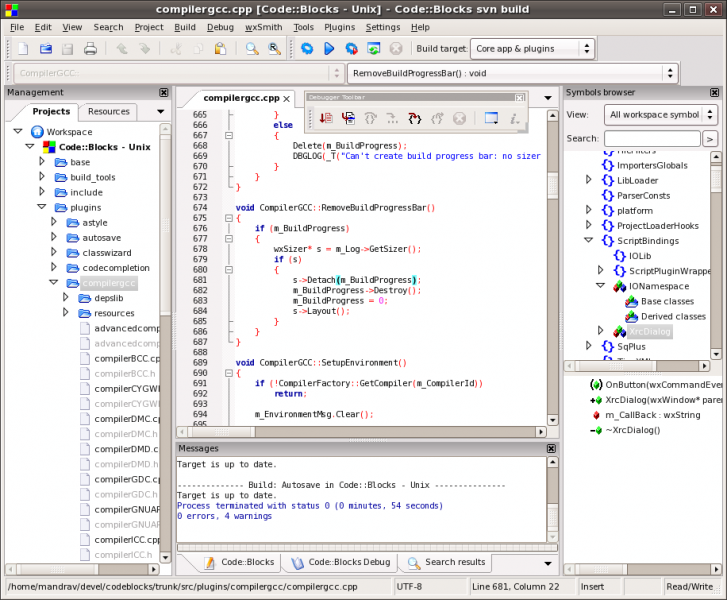
\includegraphics[width=0.6\linewidth]{images/cb}
%		\caption{contoh tampilan Code::Blocks}
%	\end{figure}
%
%	Berikut instalasi:
%	\begin{itemize}
%		\item Windows.
%		\begin{itemize}
%			\item Buka alamat \url{http://www.codeblocks.org/downloads/26}.
%			\item Klik file codeblocks-17.12mingw-setup.exe.
%			\item Tunggu proses download selesai.
%			\item Jalankan file codeblocks-17.12mingw-setup.exe untuk instalasi.
%		\end{itemize}
%	
%		\item Ubuntu/Debian.
%		\begin{itemize}
%			\item Buka Terminal (pastikan terhubung internet).
%			\item Masukkan perintah.
%				\begin{minted}[frame=lines,fontsize=\footnotesize]{bash}
%sudo apt-get install codeblocks build-essential
%				\end{minted}
%			\item Tunggu proses selesai.
%		\end{itemize}
%	
%		\item Fedora.
%		\begin{itemize}
%			\item Buka Terminal (pastikan terhubung internet).
%			\item Masukkan perintah.
%				\begin{minted}[frame=lines,fontsize=\footnotesize]{bash}
%sudo dnf groupinstall 'Development Tools'
%sudo dnf install codeblocks
%				\end{minted}
%			\item Tunggu proses selesai.
%		\end{itemize}
%	
%		\item Arch-Linux.
%		\begin{itemize}
%			\item Buka Terminal (pastikan terhubung internet).
%			\item Masukkan perintah.
%			\begin{minted}[frame=lines,fontsize=\footnotesize]{bash}
%sudo pacman -S codeblocks base-devel 
%			\end{minted}
%			\item Tunggu proses selesai.
%		\end{itemize}
%
%	\end{itemize}
%
%	\subsubsection{GCC AVR}
%	GCC adalah software kompilasi gratis dan bebas untuk chip AVR.
%	GCC (GNU C Compiler) bertugas mengkompilasi kode sumber menjadi file \textit{binary} yang siap dijalankan atau di-\textit{download} ke dalam chip.
%
%	Berikut instalasi:
%	\begin{itemize}
%		\item Windows.
%		\begin{itemize}
%			\item Download file instalasi di alamat:
%			\begin{itemize}
%				\item Windows x86 (32bit):\\
%				\url{http://blog.zakkemble.net/download/avr-gcc-8.3.0-x86-mingw.zip}
%				\item Windows x64 (64bit):\\
%				\url{http://blog.zakkemble.net/download/avr-gcc-8.3.0-x64-mingw.zip}
%			\end{itemize}
%			\item Extrak file yang sudah di download.
%			\item Masukkan alamat kompiler dalam \textit{binary path} milik Windows.
%		\end{itemize}
%	
%		\item Ubuntu/Debian.
%		\begin{itemize}
%			\item Buka Terminal (pastikan terhubung internet).
%			\item Masukkan perintah.
%			\begin{minted}[frame=lines,fontsize=\footnotesize]{bash}
%sudo apt-get install gcc-avr binutils-avr avr-libc
%			\end{minted}
%			\item Tunggu proses selesai.
%		\end{itemize}
%		
%		\item Fedora.
%		\begin{itemize}
%			\item Buka Terminal (pastikan terhubung internet).
%			\item Masukkan perintah.
%			\begin{minted}[frame=lines,fontsize=\footnotesize]{bash}
%sudo dnf install avr-binutils avr-gcc avr-libc
%			\end{minted}
%			\item Tunggu proses selesai.
%		\end{itemize}
%		
%		\item Arch-Linux.
%		\begin{itemize}
%			\item Buka Terminal (pastikan terhubung internet).
%			\item Masukkan perintah.
%			\begin{minted}[frame=lines,fontsize=\footnotesize]{bash}
%sudo pacman -S avr-binutils avr-gcc avr-lib 
%			\end{minted}
%			\item Tunggu proses selesai.
%		\end{itemize}
%			
%	\end{itemize}
%
%	\subsubsection{Downloader}
%	Download adalah software bantu untuk download (memasukkan) binary hasil kompilasi ke dalam chip.
%	Tersedia banyak software tergantung tipe hardware downloader yang dipakai.
%	Untuk kursus ini, digunakan downloader berbasis UASAsp, maka software downloader yang digunakan adalah
%	Khazama untuk Windows dan avrdude (AVR Downloader/UploaDEr) untuk selain Windows.
%	
%	Berikut instalasi:
%	\begin{itemize}
%		\item Windows
%		\begin{figure}[H]
%			\centering
%			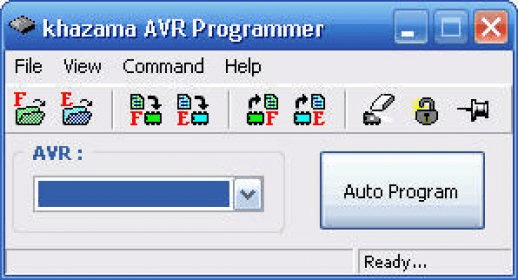
\includegraphics[width=0.4\linewidth]{images/khazama}
%			\caption{contoh tampilan Khazama}
%		\end{figure}
%		\begin{itemize}
%			\item Download file instalasi Khazama 1.6 di alamat \url{http://khazama.com/project/programmer/KhazamaAVRProgrammer162.rar}.
%			\item Ekstrak file yang di download dan jalankan file installernya.
%		\end{itemize}
%	
%		\item Ubuntu/Debian.
%		\begin{itemize}
%			\item Buka Terminal (pastikan terhubung internet).
%			\item Masukkan perintah.
%			\begin{minted}[frame=lines,fontsize=\footnotesize]{bash}
%sudo apt-get install avrdude
%			\end{minted}
%			\item Tunggu proses selesai.
%		\end{itemize}
%		
%		\item Fedora.
%		\begin{itemize}
%			\item Buka Terminal (pastikan terhubung internet).
%			\item Masukkan perintah.
%			\begin{minted}[frame=lines,fontsize=\footnotesize]{bash}
%sudo dnf install avrdude
%			\end{minted}
%			\item Tunggu proses selesai.
%		\end{itemize}
%		
%		\item Arch-Linux.
%		\begin{itemize}
%			\item Buka Terminal (pastikan terhubung internet).
%			\item Masukkan perintah.
%			\begin{minted}[frame=lines,fontsize=\footnotesize]{bash}
%sudo pacman -S avrdude
%			\end{minted}
%			\item Tunggu proses selesai.
%		\end{itemize}
%
%	\end{itemize}
%
%	\subsubsection{Simul-IDE}
%	
%	Dalam kursus ini, untuk awal pelatihan, digunakan Simulator untuk menjalankan dan menguji program AVR yang dibuat.
%	Simulator yang dipilih disini adalah Simul-IDE. 
%	Simul-IDE adalah simulator rangkaian elektronik Digital/Analog sederhana yang dapat berjalan secara \textit{real-time}.
%	Simul-IDE dapat mendukung microcontroller seperti chip seri AVR ataupun PIC.
%	
%	\begin{figure}[H]
%		\centering
%		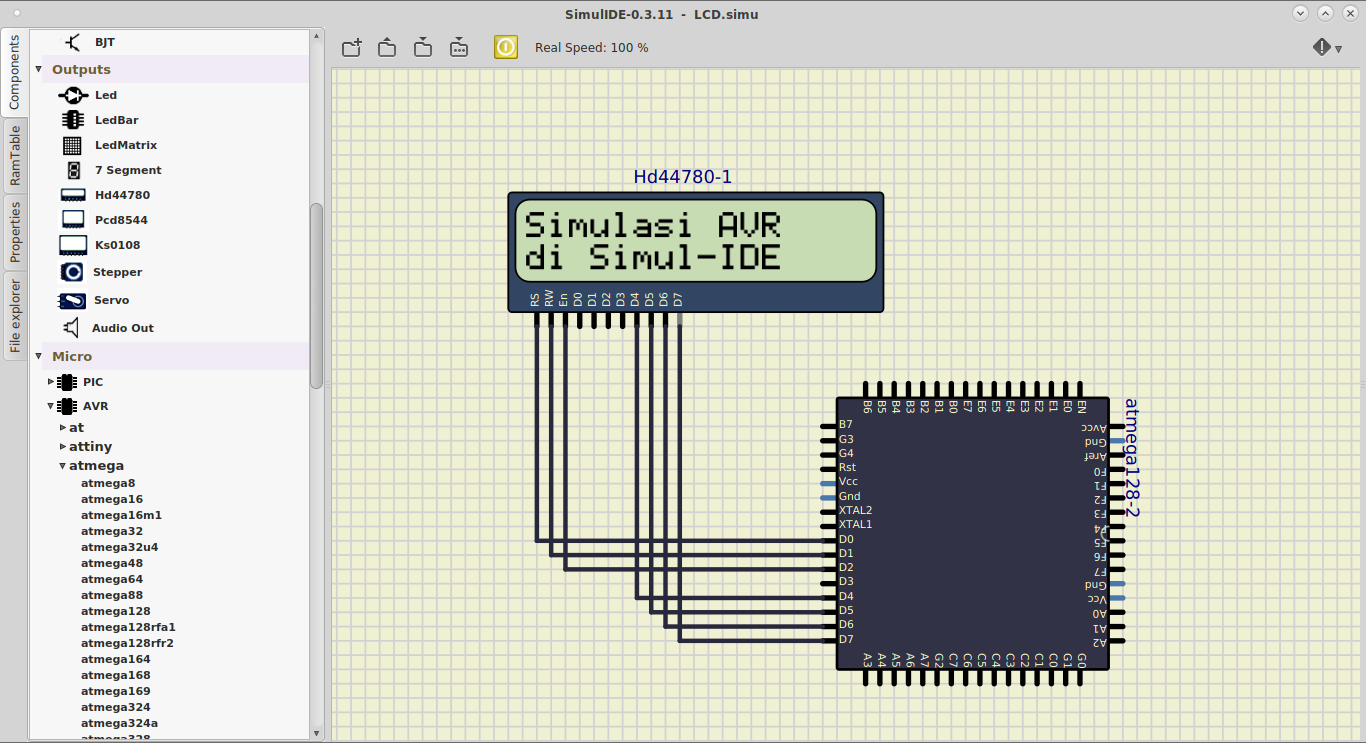
\includegraphics[width=0.6\linewidth]{images/simul}
%		\caption{contoh tampilan Simul-IDE}
%	\end{figure}
%
%	Berikut untuk instalasi:
%	\begin{itemize}
%		\item Windows
%		\begin{itemize}
%			\item Buka alamat Simul-IDE:\\
%			\url{https://sourceforge.net/projects/simulide/files/SimulIDE_0.3.10/SimulIDE_0.3.10_SR1-Win32.zip/download}
%			\item Ekstrak file yang sudah di download.
%			\item Jalankan file \textbf{run\_simulide.bat}.
%		\end{itemize}
%	
%		\item Ubuntu/Debian.
%		\begin{itemize}
%			\item Buka Terminal (pastikan terhubung internet).
%			\item Masukkan perintah.
%			\begin{minted}[frame=lines,fontsize=\footnotesize]{bash}
%sudo apt-get install simulide simavr
%			\end{minted}
%			\item Tunggu proses selesai.
%			\item Buka terminal dimana project AVR berada.
%			\item Masukkan perintah:
%			\begin{minted}[frame=lines,fontsize=\footnotesize]{bash}
%simulide
%			\end{minted}
%		\end{itemize}
%	
%		\item Fedora.
%		\begin{itemize}
%			\item Buka Terminal (pastikan terhubung internet).
%			\item Masukkan perintah.
%			\begin{minted}[frame=lines,fontsize=\footnotesize]{bash}
%sudo dnf install simulide simavr
%			\end{minted}
%			\item Tunggu proses selesai.
%			\item Buka terminal dimana project AVR berada.
%			\item Masukkan perintah:
%			\begin{minted}[frame=lines,fontsize=\footnotesize]{bash}
%simulide
%			\end{minted}
%		\end{itemize}
%	
%		\item Arch Linux.
%		\begin{itemize}
%			\item Buka Terminal (pastikan terhubung internet).
%			\item Masukkan perintah.
%			\begin{minted}[frame=lines,fontsize=\footnotesize]{bash}
%sudo pacman -S simavr
%			\end{minted}
%			\item Tunggu proses selesai.
%			\item Download resep AUR di \url{https://aur.archlinux.org/cgit/aur.git/snapshot/simulide.tar.gz}
%			\item Ekstrak file tersebut dan buka terminal di alamat tersebut.
%			\item Masukkan perintah:
%			\begin{minted}[frame=lines,fontsize=\footnotesize]{bash}
%makepkg -sir
%			\end{minted}
%			\item Tunggu proses instalasi selesai
%			\item Buka terminal dimana project AVR berada.
%			\item Masukkan perintah:
%			\begin{minted}[frame=lines,fontsize=\footnotesize]{bash}
%simulide
%			\end{minted}
%		\end{itemize}
%		
%	\end{itemize}
%
%	\subsubsection{KiCad}
%	KiCad adalah software bebas dan gratis untuk membantu merancang circuit elektronik.
%	KiCad menyediakan fitur olah skematik, layout PCB, dan 3D visualisasi.
%	
%	\begin{figure}[H]
%		\centering
%		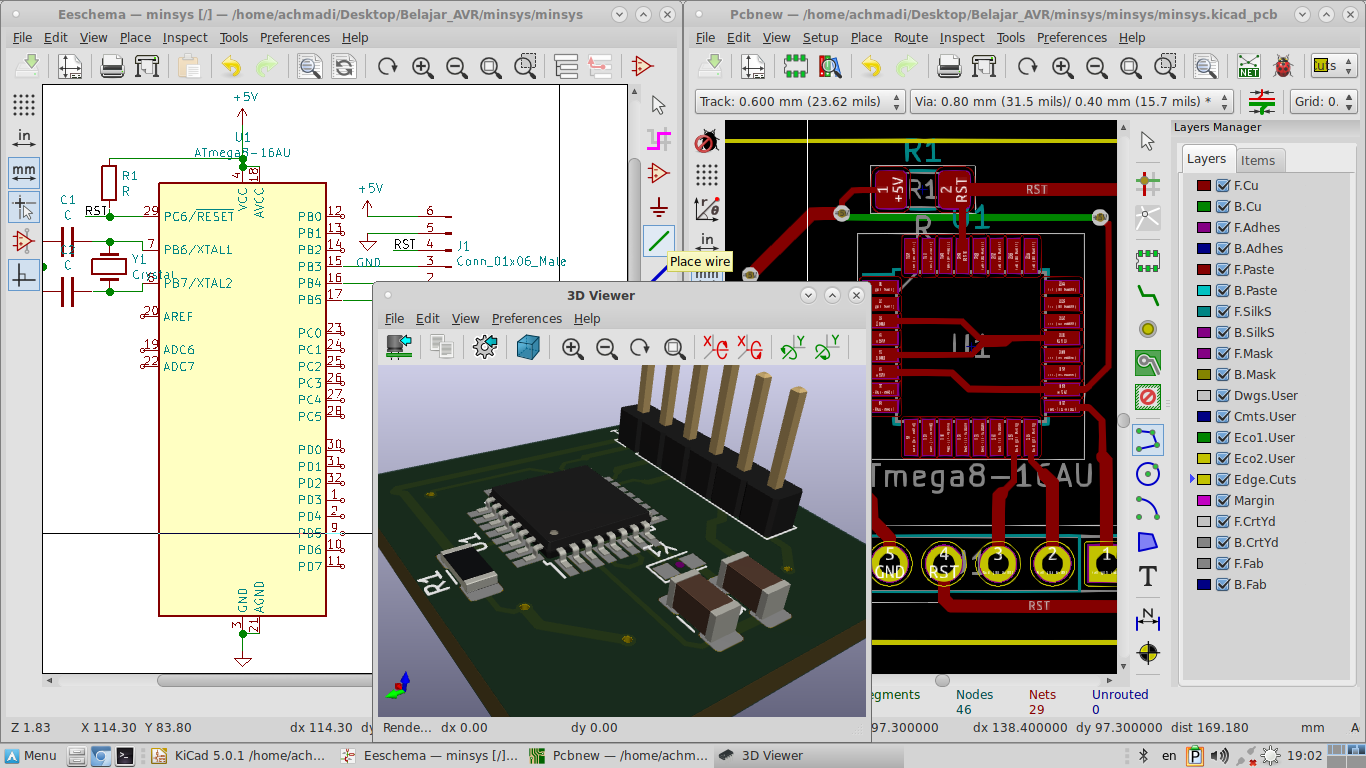
\includegraphics[width=0.6\linewidth]{images/kicad}
%		\caption{contoh tampilan KiCAD}.
%	\end{figure}
%
%	Berikut untuk instalasi:
%	\begin{itemize}
%		\item Windows
%		\begin{itemize}
%			\item Buka alamat \url{http://kicad-pcb.org/download/windows/}
%			\item Pilih dan download file instalasi sesuai laptop/komputer anda.
%			\item Jalankan file instalasi.
%		\end{itemize}
%	
%		\item Ubuntu/Debian.
%		\begin{itemize}
%			\item Buka Terminal (pastikan terhubung internet).
%			\item Masukkan perintah.
%			\begin{minted}[frame=lines,fontsize=\footnotesize]{bash}
%sudo add-apt-repository ppa:js-reynaud/kicad-5
%sudo apt-get update
%sudo apt-get install kicad
%			\end{minted}
%			\item Tunggu proses selesai.
%		\end{itemize}
%		
%		\item Fedora.
%		\begin{itemize}
%			\item Buka Terminal (pastikan terhubung internet).
%			\item Masukkan perintah.
%			\begin{minted}[frame=lines,fontsize=\footnotesize]{bash}
%sudo dnf install kicad kicad-packages3d
%			\end{minted}
%			\item Tunggu proses selesai.
%		\end{itemize}
%		
%		\item Arch Linux.
%		\begin{itemize}
%			\item Buka Terminal (pastikan terhubung internet).
%			\item Masukkan perintah.
%			\begin{minted}[frame=lines,fontsize=\footnotesize]{bash}
%sudo pacman -S kicad kicad-library kicad-library-3d
%			\end{minted}
%			\item Tunggu proses selesai.
%		\end{itemize}
%		
%	\end{itemize}
%
%	\newpage
%	\subsection{Hardware}
%	
%	Untuk hardware, kebutuhan pokok dalam membangun aplikasi ATMega hanyalah 2 saja, yaitu: Downloader dan Minimum-System 
%	
%	\subsubsection{Downloader}
%	Downloader adalah hardware yang digunakan untuk memasukkan program dalam chip.
%	Tipe downloader yang digunakan disini adalah USBAsp dimana baik skematik maupun firmware yang digunakan bersifat open-source.
%	USBAsp secara mendasar hanya membutuhkan:
%	\begin{itemize}
%		\item ATMega48, ATMega8, atau ATMega88
%		\item Clock 12MHz atau lebih
%		\item 2 PIN untuk jalur VCC dan GND
%		\item 4 PIN untuk jalur SPI (SS, MOSI, MISO, dan SCK)
%		\item 4 PIN untuk jalur USB (VCC, GND, D+, dan D-)
%	\end{itemize}
%	Project USBAsp dapat anda temukan di alamat \url{https://www.fischl.de/usbasp/}.
%	
%	\begin{figure}[H]
%		\centering
%		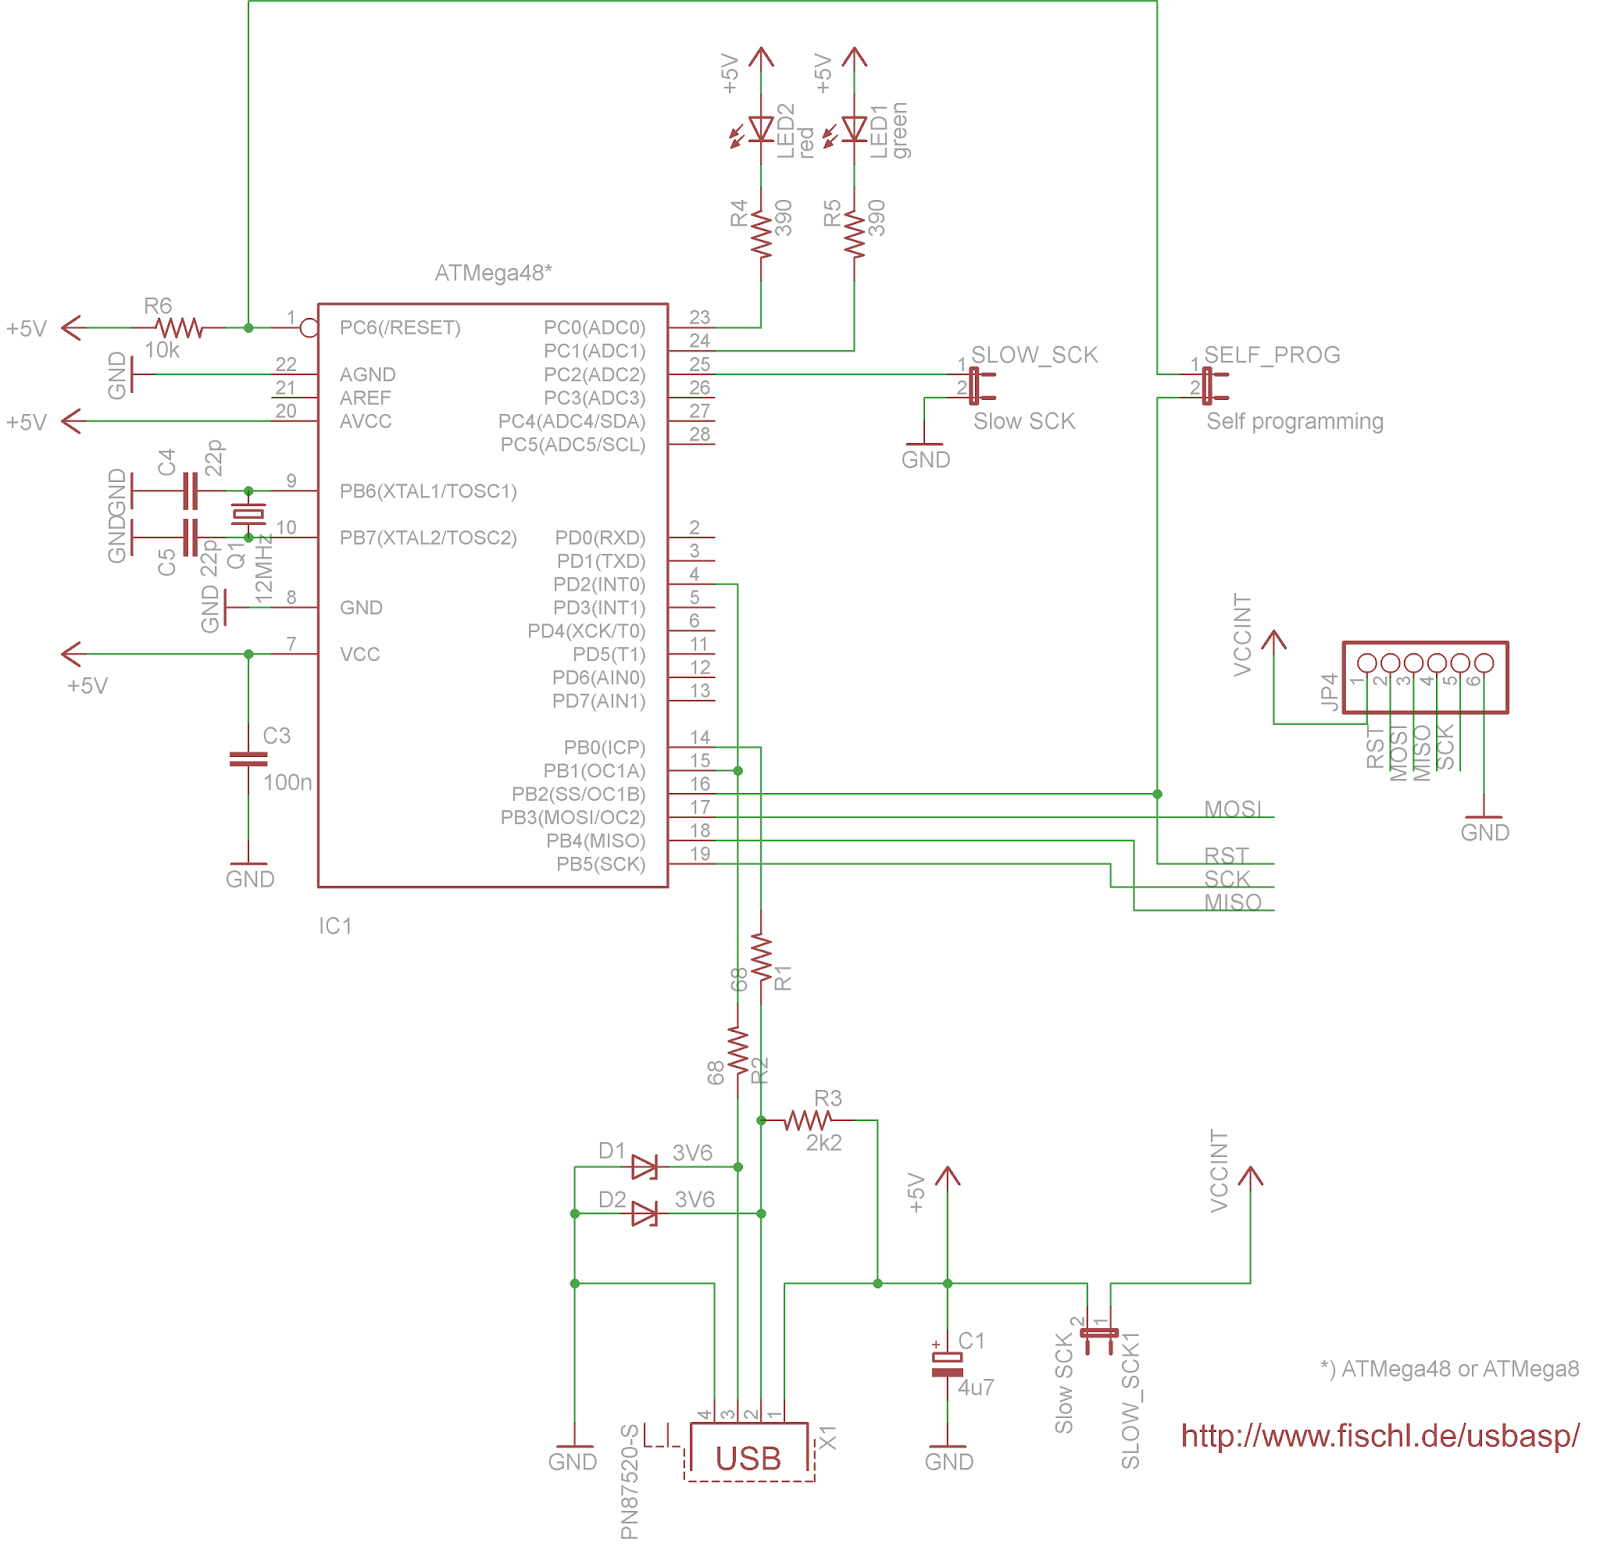
\includegraphics[width=0.6\linewidth]{images/usbasp}
%		\caption{contoh skematik USBAsp}
%	\end{figure}
%
%	Sedangkan untuk hardware dapat anda beli di pasaran dengan harga terjangkau atau anda dapat merakit sendiri.
%	
%	\begin{figure}[H]
%		\centering
%		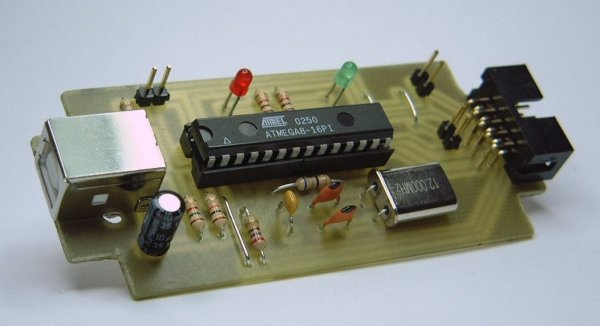
\includegraphics[width=0.6\linewidth]{images/usbasphard}
%		\caption{contoh USBAsp murah meriah}
%	\end{figure}
%
%	\textbf{Advance}: Selain menggunakan USBAsp fisik, anda dapat juga menanamkan \textit{virtual} downloader USBAsp kedalam bagian \textit{bootloader} ATMega.
%	Keuntungannya anda tidak lagi perlu USBAsp fisik terpisah dengan Minimum-System,
%	namun kekurangannya adalah alamat aplikasi berpindah ke alamat bootloader sehingga terkadang memory tidak sampai alamat aplikasi.
%	Project ini dikenal dengan USBAspLoader dan dapat anda temukan di \url{https://www.obdev.at/products/vusb/usbasploader.html}.
%	
%	\subsubsection{Minimum-System}
%	Minimum-System didefiniskan sebagai rangkaian dasar agar chip ATMega dapat berjalan.
%	Pada dasarnya ATMega hanya membutuhkan:
%	\begin{itemize}
%		\item Power VCC (5v) dan GND (0v). Power ini bisa didapat dari tegangan USB atau output regulator 7805/LM2569s.
%		\item 5 PIN untuk download via SPI (GND, RST, MOSI, MISO, dan SCK) jika ingin didownload \textit{on-board}.
%		\item Crystal (XTALL) atau RTC jika sumber Clock ATMega di set eksternal.
%	\end{itemize}
%
%	\begin{figure}[H]
%		\centering
%		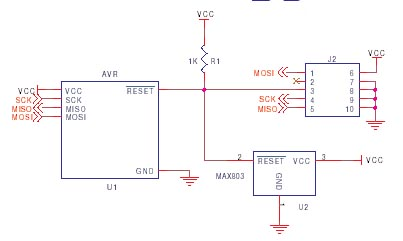
\includegraphics[width=0.6\linewidth]{images/minsys}
%		\caption{contoh diagram dasar Minimum-System}
%	\end{figure}
%
%	Berdasarkan rangkaian dasar ini, anda dapat menambahkan beragam komponen lain sesuai kebutuhan anda.
%	Jika anda tidak waktu untuk membangun Minimum-System sendiri, anda dapat membelinya di pasaran dengan beragam harga dan spesifikasi.
%	
%	\begin{figure}[H]
%		\centering
%		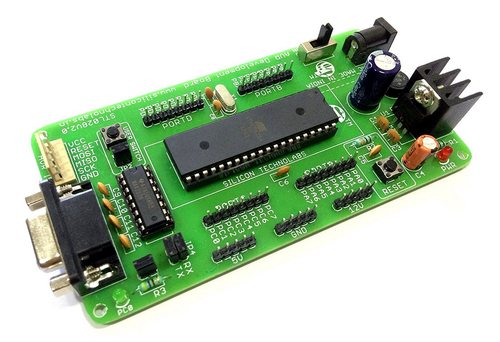
\includegraphics[width=0.6\linewidth]{images/minsyshard}
%		\caption{contoh fisik Minimum-System yang dilengkapi RS-232 dan regulator 5v}
%	\end{figure}

	\newpage
	\section{Bahasa C}
	
	\subsection{Requirement}
	
	Berikut Software yang dibutuhkan.
	
	\subsubsection{Code::Blocks}
	Code::Blocks adalah suatu program lingkungan pengembangan terpadu bebas, gratis, bersumber terbuka dan lintas platform.
	Program yang ditulis dalam C++ beserta wxWidgets untuk GUI-nya ini bisa digunakan bersama dengan berbagai macam kompilator, contohnya GCC dan CLang.
	Peralatannya yang tersedia tergantung dari "plugin" yang ada dipasang.
	Sekarang ini, Code::Blocks lebih tersedia sebagai perangkat pengembangan dalam bahasa C dan C++, walaupun program ini juga bisa disesuaikan, 
	dan mungkin akan membutuhkan pemasangan tambahan, untuk pengembangan perangkat lunak ARM, AVR, Fortran, GLFW, GLUT, GTK+,  MATLAB, OGRE, OpenGL, Qt, atau SDL.
	Code::Blocks tersedia di sistem operasi Windows, Linux, Mac OS X dan FreeBSD.
	\begin{figure}[H]
		\centering
		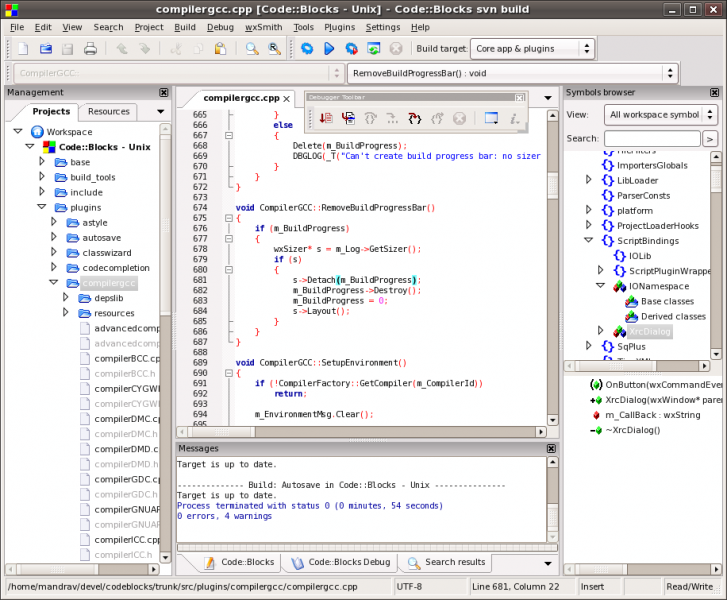
\includegraphics[width=0.6\linewidth]{images/cb}
		\caption{contoh tampilan Code::Blocks}
	\end{figure}
	
	Berikut instalasi:
	\begin{itemize}
		\item Windows.
		\begin{itemize}
			\item Buka alamat \url{http://www.codeblocks.org/downloads/26}.
			\item Klik file codeblocks-17.12mingw-setup.exe.
			\item Tunggu proses download selesai.
			\item Jalankan file codeblocks-17.12mingw-setup.exe untuk instalasi.
		\end{itemize}
		
		\item Ubuntu/Debian.
		\begin{itemize}
			\item Buka Terminal (pastikan terhubung internet).
			\item Masukkan perintah.
			\begin{minted}[frame=lines,fontsize=\footnotesize]{bash}
			sudo apt-get install codeblocks build-essential
			\end{minted}
			\item Tunggu proses selesai.
		\end{itemize}
		
		\item Fedora.
		\begin{itemize}
			\item Buka Terminal (pastikan terhubung internet).
			\item Masukkan perintah.
			\begin{minted}[frame=lines,fontsize=\footnotesize]{bash}
			sudo dnf groupinstall 'Development Tools'
			sudo dnf install codeblocks
			\end{minted}
			\item Tunggu proses selesai.
		\end{itemize}
		
		\item Arch-Linux.
		\begin{itemize}
			\item Buka Terminal (pastikan terhubung internet).
			\item Masukkan perintah.
			\begin{minted}[frame=lines,fontsize=\footnotesize]{bash}
			sudo pacman -S codeblocks base-devel 
			\end{minted}
			\item Tunggu proses selesai.
		\end{itemize}
		
	\end{itemize}
	
	\newpage	
	\subsection{Pengenalan}
	Bahasa pemrograman C merupakan salah satu bahasa pemrograman komputer. Dibuat pada tahun 1972 oleh Dennis Ritchie untuk Sistem Operasi Unix di Bell Telephone Laboratories.
	
	Meskipun C dibuat untuk memprogram sistem dan jaringan komputer namun bahasa ini juga sering digunakan dalam mengembangkan software aplikasi.
	C juga banyak dipakai oleh berbagai jenis platform sistem operasi dan arsitektur komputer, bahkan terdapat beberepa compiler yang sangat populer telah tersedia.
	C secara luar biasa memengaruhi bahasa populer lainnya, terutama C++ yang merupakan extensi dari C.
	
	\subsubsection{Kompilasi}
	Kompilasi adalah proses mengumpulkan dan mengubah kode sumber menjadi file yang bisa dijalankan.
	Software/Firmware memiliki 2 bentuk yaitu kode sumber (\textit{source}) dan \textit{binary}.
	Source dapat dibaca oleh manusia, namun belum bisa dimengerti oleh CPU.
	Sebaliknya, binary tidak bisa dipahami manusia, namun bisa dipahami CPU dan dijalankan isinya. 
	Berikut secara ringkas diagram kompilasi:
	
	\begin{figure}[H]
		\begin{center}
			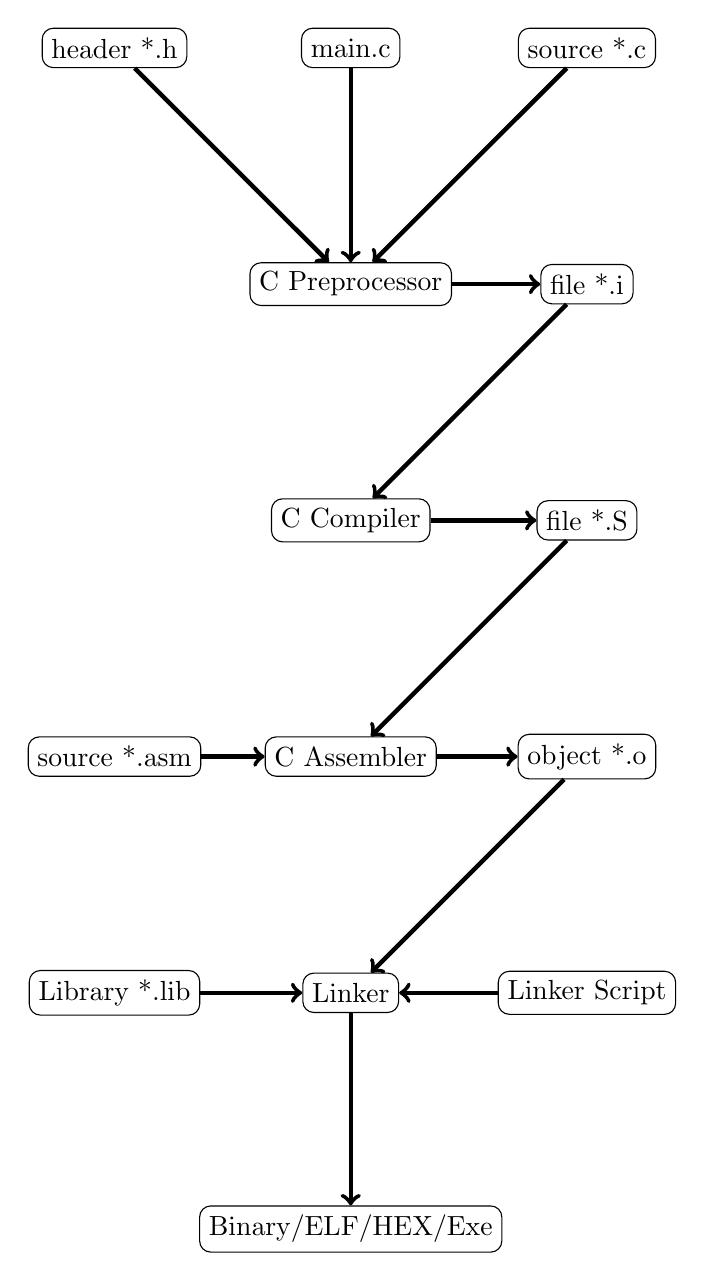
\begin{tikzpicture}[node distance=3cm]
			\node (mainc) [squared] {main.c};
			\node (cheader) [squared,left of=mainc] {header *.h};
			\node (csource) [squared,right of=mainc] {source *.c};
			\node (preproc)[squared,below of=mainc]{C Preprocessor};
			\node (cproc)[squared,right of=preproc]{file *.i};
			%-----------------------------------------------
			\node (cc) [squared,below of=preproc]{C Compiler};
			\node (casm) [squared,right of=cc]{file *.S};
			%-----------------------------------------------
			\node (asm) [squared,below of=cc]{C Assembler};
			\node (asmsource)[squared,left of=asm]{source *.asm};
			\node (obj)[squared,right of=asm]{object *.o};
			%-----------------------------------------------
			\node (linker) [squared,below of=asm]{Linker};
			\node (library) [squared,left of=linker]{Library *.lib};
			\node (linkscr) [squared,right of=linker]{Linker Script};
			%-----------------------------------------------
			\node (binary) [squared,below of=linker]{Binary/ELF/HEX/Exe};
			
			%-----------------------------------------------
			%-----------------------------------------------
			
			\draw [connect] (mainc) -- (preproc);
			\draw [connect] (cheader) -- (preproc);
			\draw [connect] (csource) -- (preproc);
			\draw [connect] (preproc) -- (cproc);
			\draw [connect] (cproc) -- (cc);
			\draw [connect] (cc) -- (casm);
			\draw [connect] (casm) -- (asm);
			\draw [connect] (asmsource) -- (asm);
			\draw [connect] (asm) -- (obj);
			\draw [connect] (obj) -- (linker);
			\draw [connect] (library) -- (linker);
			\draw [connect] (linkscr) -- (linker);
			\draw [connect] (linker) -- (binary);
			\end{tikzpicture}
			\caption{Diagram Proses Kompilasi}
		\end{center}
	\end{figure}

	\newpage
	\subsubsection{Hello World}
	Bahasa C secara umum memiliki 4 bagian wajib, yaitu:
	\begin{itemize}
		\item Preprocessor
		\item Functions
		\item Variables
		\item Expressions atau Operation.
	\end{itemize}

	Setiap satu baris kode pemrograman yang kita buat disebut sebagai \textit{statement}.
	Statement dapat berupa salah satu atau gabungan dari komponen di atas.
	Setiap baris statement diakhiri dengan tanda titik koma (;).
	
	Berikut adalah contoh dasar yang dapat dijalankan di Code::Blocks.
	\begin{enumerate}
		\item Buka Code::Blocks.
		\item Buat project baru.
		\begin{figure}[H]
			\centering
			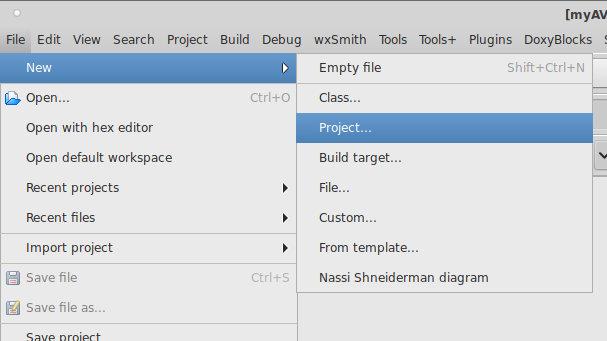
\includegraphics[width=0.5\linewidth]{images/c_cb_0}
			\caption{membuat project baru}
		\end{figure}
		\item Pilih Empty Project.
		\begin{figure}[H]
			\centering
			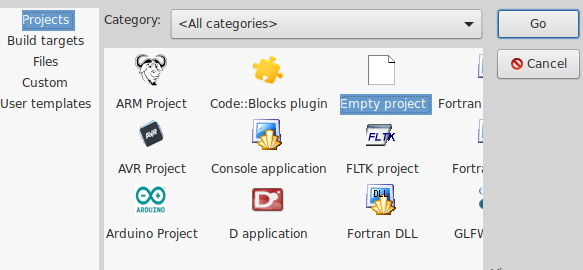
\includegraphics[width=0.4\linewidth]{images/c_cb_1}
			\caption{membuat project kosong}
		\end{figure}
		\item Isi nama project.
		\begin{figure}[H]
			\centering
			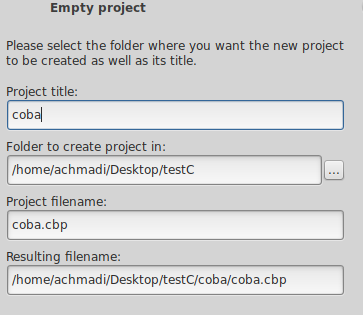
\includegraphics[width=0.35\linewidth]{images/c_cb_2}
			\caption{nama dan tempat project}
		\end{figure}
		\item Pilih compiler \textbf{GNU GCC} dan isi build target \textbf{all} seperti dibawah.
		\begin{figure}[H]
			\centering
			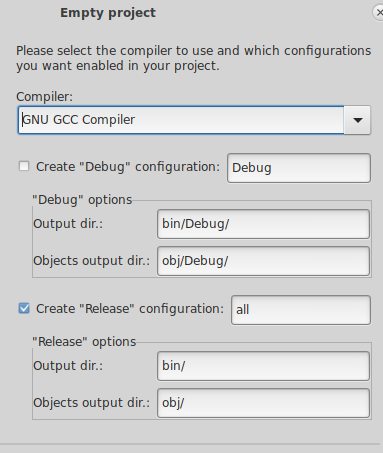
\includegraphics[width=0.35\linewidth]{images/c_cb_3}
			\caption{pilih compiler}
		\end{figure}
		\item Buat File baru
		\begin{figure}[H]
			\centering
			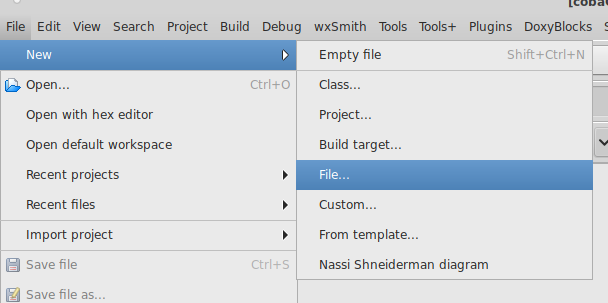
\includegraphics[width=0.4\linewidth]{images/c_cb_4}
			\caption{buat file baru}
		\end{figure}
		\item Pilih file C/C++ Sources
		\begin{figure}[H]
			\centering
			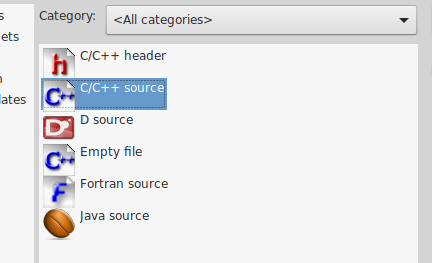
\includegraphics[width=0.4\linewidth]{images/c_cb_5}
			\caption{C/C++ source}
		\end{figure}
	
		\item Pilih tipe C
		\begin{figure}[H]
			\centering
			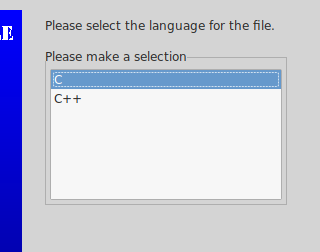
\includegraphics[width=0.35\linewidth]{images/c_cb_6}
			\caption{C source}
		\end{figure}
		\item isi alamat folder project tadi diakhiri dengan \textbf{main.c}.
		Jangan lupa centang \textbf{all} untuk menambahkan file ke build target.
		\begin{figure}[H]
			\centering
			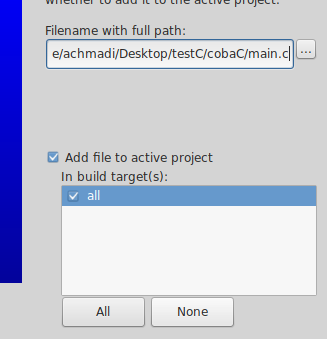
\includegraphics[width=0.35\linewidth]{images/c_cb_7}
			\caption{nama dan alamat file}
		\end{figure}
	    
		\item hasil akhir \textbf{main.c}.
		\begin{figure}[H]
			\centering
			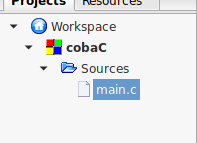
\includegraphics[width=0.35\linewidth]{images/c_cb_8}
			\caption{file main.c}
		\end{figure}
	
		\item pastikan file C sudah masuk ke build target.
		Klik menu \textbf{Properties} -> tab \textbf{Build Targets}.
		\begin{figure}[H]
			\centering
			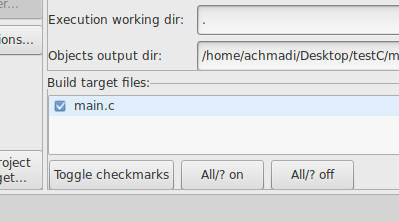
\includegraphics[width=0.35\linewidth]{images/c_cb_9}
			\caption{build target}
		\end{figure}
	
		\item masukkan kode berikut.
		Tips: Manfaatkan Code Compeletion.
		\begin{minted}[frame=lines,fontsize=\footnotesize]{c}
#include <stdio.h>

int main() {
	printf("Hello, World! \n");
	return 0;
}
		\end{minted}
		\item Tekan menu \textbf{Build}->\textbf{Build and Run}.
		\begin{figure}[H]
			\centering
			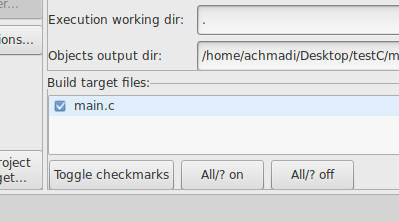
\includegraphics[width=0.4\linewidth]{images/c_cb_9}
			\caption{Build and Run}
		\end{figure}
			
	\end{enumerate}

	\subsubsection{Komentar}
	Komentar adalah bagian dari kode sumber yang bukan bagian dari pemrograman dan tidak dikompilasi compiler.
	Komentar ini berfungsi sebagai penanda, dokumentasi, penjelasan, atau apa saja yang dapat membantu memahami source yang ditulis.
	Bisa juga sekedar "non-aktifkan" sebagian kode.\\
	Berikut contoh komentar:
	\begin{itemize}
		\item Per Baris
		\begin{minted}[frame=lines,fontsize=\footnotesize]{c}
// contoh komentar
unsigned int vt=0; //sebelah ini bukan komentar
// per baris
		\end{minted}
		
		\item Per Block
		\begin{minted}[frame=lines,fontsize=\footnotesize]{c}
/* contoh komentar
unsigned int vt=0; (sebelah ini ikut jadi komentar)
per baris */
		\end{minted}
	\end{itemize}

	\newpage
	\subsection{Variabel}
	Variablel adalah entitas yang menyimpan suatu nilai dalam memory.
	Beberapa yang perlu dipahami tentang variabel.
	
	\subsubsection{Tipe Data}
	Tipe data dalam bahasa C diukur dengan satuan \textbf{bit}.
	Nilai 1 bit adalah nilai terkecil dalam memory yang bisa diisi antara 1 atau 0 (salah satu).
	Berikut satuan tipe data yang sering dipakai:
	\begin{itemize}
		\item Bit. Satuan terkecil yang hanya berisi 1 atau 0
		\item Nibble. Senilai dengan 4bit.
		\item Byte. Senilai dengan 8bit.
	\end{itemize}
	
	Selanjutnya dalam alokasi variable dalam memory, dikenal istilah tipe data.
	Tipe data adalah deklarasi jenis variable berdasarkan ukurannya.
	Setiap tipe data memiliki ukuran maximal yang jika nilai nya melewatinya akan terjadi \textit{overflow} (kembali ke 0).
	Berikut tipe data yang umum:
	\begin{table}[H]
		\begin{tabular}{|l|l|l|l|l}
			\cline{1-4}
			\textbf{name}      & \textbf{type}          & \textbf{bit-size} & \textbf{range} &  \\ \cline{1-4}
			character & unsigned char & 8  & 0$\sim$255           &  \\ \cline{1-4}
			character & char          & 8  & -127$\sim$128        &  \\ \cline{1-4}
			integer   & unsigned int  & 16 & 0$\sim$65,535        &  \\ \cline{1-4}
			integer   & int  		  & 16 & -32,768$\sim$32,767  &  \\ \cline{1-4}
			long	  & unsigned long & 32 & 0$\sim$4,294,967,295 &  \\ \cline{1-4}
			long	  & long 		  & 32 & $\pm$2,147,483,647	  &  \\ \cline{1-4}
			float	  & float 		  & 32 & $\pm$2,147,483,647	  &  \\ \cline{1-4}
			double	  & double 		  & 64 & $\pm$9,223,372,036,854,775,807	&  \\ \cline{1-4}
		\end{tabular}
	\end{table}
	Untuk tipe double dan float, mampu menyimpan bilangan \textit{floating-point} (decimal).
	Akan tetapi standar floating-point setiap chip arsitektur berbeda-beda sehingga perlu diperhatikan.
	
	\subsubsection{Deklarasi}
	Tujuan setelah mengenal tipe data adalah untuk mendeklarasikan tipe variabel sesuai kebutuhan.
	Dalam bahasa C/C++, variable wajib dideklarasikan terlebih dahulu agar sistem dapat memesan ukuran memori secara pas.
	Pola deklarasi variable:
	\begin{minted}[frame=lines,fontsize=\footnotesize]{c}
<asal> <rentang> <tipedata> variabel;
	\end{minted}
	Penjelasan:
	\begin{itemize}
		\item <asal> adalah penanda asal variabel. Pilihannya adalah \textbf{external} dimana variabel tersebut dideklarasikan di file source lain,
		namun perlu dideklarasi ulang agar dikenali (tanpa ada pengisian nilai).
		Atau \textbf{kosong} saja jika deklarasi variabel di file source itu sendiri.
		\item <rentang> adalah tipe rentang yang dipakai.
		Pilihannya adalah \textbf{unsigned} yaitu dari 0 hingga maximal.
		Dan \textbf{signed} atau \textbf{kosong} saja untuk minus setengah maximal hingga plus setengah maximal.
		\item <tipedata> adalah tipe data sesuai rentang.
		\item variabel adalah nama variable dengan aturan:
		\begin{itemize}
			\item tidak diawali angka, tapi boleh underscore (\_).
			\item tidak boleh ada spasi,koma,titik, tapi boleh underscore (\_).
			\item tidak konflik nama dengan yang lain di lingkungan pemrograman.
		\end{itemize}
	\end{itemize}

	Sebagai contoh:
	\begin{minted}[frame=lines,fontsize=\footnotesize]{c}
extern int fooalien; // boleh
extern int fooalien=5; // tidak boleh

unsigned int foo;
foo = 5;
foo = -5; //tidak boleh

int foomin;
foomin = -5;
	\end{minted}
	
	\subsubsection{TypeCast}
	TypeCast adalah mengubah tipe akhir suatu operasi dari satu tipe data ke tipe data lain.
	Proses ini biasanya digunakan untuk mencegah overflow.
	Pola umum:
	\begin{minted}[frame=lines,fontsize=\footnotesize]{c}
variable = (type_data) statement;
	\end{minted}
	Contoh
	\begin{minted}[frame=lines,fontsize=\footnotesize]{c}
unsigned char a,b;
unsigned int c;

a=b=250;
c=(unsigned int)a+b;
	\end{minted}
	
	\subsubsection{Konstanta}
	Konstanta adalah nilai atau bilangan tetap yang nanti bisa dimasukkan kedalam variabel.
	Konstanta memiliki beberapa cara penulisan yang disesuaikan kebutuhan.
	Yang umum dipakai antara lain
	\begin{itemize}
		\item Decimal.Setiap digit merepresentasikan kelipatan 10.
		Penulisan menggunakan angka pada umumnya.
		Contoh. Bilangan 500 untuk variabel integer.
		\begin{minted}[frame=lines,fontsize=\footnotesize]{c}
unsigned int a=500;
		\end{minted}
		
		\item Biner.Setiap digit merepresentasikan kelipatan 1 bit.
		Penulisan menggunakan awalan '0b'.
		Contoh. Bilangan 0b00001111 untuk variabel char.
		\begin{minted}[frame=lines,fontsize=\footnotesize]{c}
unsigned char a=0b00001111;
		\end{minted}
		
		\item Hexa.Setiap digit merepresentasikan kelipatan 4 bit (1 nibble).
		Penulisan menggunakan awalan '0x'.
		Contoh. Bilangan 0x0F untuk variabel char.
		\begin{minted}[frame=lines,fontsize=\footnotesize]{c}
unsigned char a=0x0F;
		\end{minted}
	\end{itemize}

	Untuk mempermudah berikut contoh tabel konversi:
	\begin{table}[H]
		\begin{tabular}{|l|l|l|l}
			\cline{1-3}
			\textbf{decimal} & \textbf{biner} & \textbf{hexa} \\ \cline{1-3}
			0 & 0b0000 & 0x0  \\ \cline{1-3}
			1 & 0b0001 & 0x1  \\ \cline{1-3}
			2 & 0b0010 & 0x2  \\ \cline{1-3}
			3 & 0b0011 & 0x3  \\ \cline{1-3}
			4 & 0b0100 & 0x4  \\ \cline{1-3}
			5 & 0b0101 & 0x5  \\ \cline{1-3}
			6 & 0b0110 & 0x6  \\ \cline{1-3}
			7 & 0b0111 & 0x7  \\ \cline{1-3}
			8 & 0b1000 & 0x8  \\ \cline{1-3}
			9 & 0b1001 & 0x9  \\ \cline{1-3}
			10 & 0b1010 & 0xA  \\ \cline{1-3}
			11 & 0b1011 & 0xB  \\ \cline{1-3}
			12 & 0b1100 & 0xC  \\ \cline{1-3}
			13 & 0b1101 & 0xD  \\ \cline{1-3}
			14 & 0b1110 & 0xE  \\ \cline{1-3}
			15 & 0b1111 & 0xF  \\ \cline{1-3}
		\end{tabular}
	\end{table}

	Catatan: dalam format internasional, pemisah ribuan adalah koma, bukan titik.
	Sementara pemisah decimal adalah titik, bukan koma.

	\newpage	
	\subsection{Operator}
	Operator adalah bagian dari bahasa pemrograman yang digunakan untuk memanipulasi isi variabel.
	
	\subsubsection{Aritmatika}
	Operator Artimatika digunakan untuk operasi Arimatik.
	Berikut tabel
	
	\begin{table}[H]
		\begin{tabular}{|l|l|l}
			\cline{1-2}
			\textbf{operator} & \textbf{arti} \\ \cline{1-2}
			* & Perkalian \\ \cline{1-2}
			/ & Pembagian \\ \cline{1-2}
			+ & Penjumlahan \\ \cline{1-2}
			- & Pengurangan \\ \cline{1-2}
			\% & Sisa \\ \cline{1-2}
		\end{tabular}
	\end{table}

	Contoh.
	\begin{minted}[frame=lines,fontsize=\footnotesize]{c}
unsigned char a,b,c;
a=6;
b=2;

c=a*b; //c=12
c=a/b; //c=3
c=a+b; //c=8
c=a-b; //c=4
c=a%b; //c=0
	\end{minted}
	
	Selanjutnya ada variasi operator aritmatik untuk operasi terhadap satu variabel.
	Pola umumnya:
	\begin{minted}[frame=lines,fontsize=\footnotesize]{c}
variabel = variabel + C
	\end{minted}

	Variabel di kanan sama-dengan adalah variabel sebelum operasi.
	Variabel di kiri sama-dengan adalah variabel hasil operasi.
	C adalah nilai atau variabel yang dioperasikan.
	Contoh
	\begin{minted}[frame=lines,fontsize=\footnotesize]{c}
unsigned char a=6;
a=a+2; //nilai akhir a menjadi 8
	\end{minted}
	
	Bentuk operasi ini dapat dipersingkat menjadi:
	\begin{minted}[frame=lines,fontsize=\footnotesize]{c}
unsigned char a=6;
a+=2; //nilai akhir a menjadi 8
	\end{minted}
	
	Jika nilai yang dipeoerasikan adalah 1, maka dapat lebih dipersingkat dengan operator \textit{increment} (++)
	Contoh:
	Bentuk operasi ini dapat dipersingkat menjadi
	\begin{minted}[frame=lines,fontsize=\footnotesize]{c}
unsigned char a=6;
a+=1; //nilai akhir a menjadi 7
a++; //nilai akhir a menjadi 7
	\end{minted}
	
	Operator seperti ini tersedia sebagai \textit{increment} ($++$) atau \textit{decrement} ($--$)
	
	\subsubsection{Hubungan}
	
	Operator Hubungan digunakan untuk pengecekan bagaimana suatu variabel terhadap suatu nilai atau variabel.
	Operator ini sering digunakan dalam pengambilan keputusan (\textit{decision}).
	Berikut Tabelnya:
	\begin{table}[H]
		\begin{tabular}{|l|l|l|l}
			\cline{1-3}
			\textbf{operator} & \textbf{contoh} & \textbf{arti} \\ \cline{1-3}
			==                & A==B            & apa A sama dengan B? \\ \cline{1-3}
			!=                & A!=B            & apa A tidak sama dengan B? \\ \cline{1-3}
			>                 & A>B             & apa A lebih dari B?  \\ \cline{1-3}
			>=                & A>=B            & apa A lebih dari atau sama dengan B?\\ \cline{1-3}
			<                 & A<B             & apa A kurang dari B? \\ \cline{1-3}
			<=                & A<=B            & apa A kurang dari atau sama dengan B? \\ \cline{1-3}
		\end{tabular}
	\end{table}

	\subsubsection{Logika}
	Operator Logika digunakan untuk pengecekan bagaimana suatu variabel terhadap suatu nilai atau variabel dari sisi logika.
	Berikut Tabelnya:
	\begin{table}[H]
		\begin{tabular}{|l|l|l|l}
			\cline{1-3}
			\textbf{operator} & \textbf{contoh} & \textbf{arti} \\ \cline{1-3}
			\&\&              & A\&\&B          & apa A dan B benar? \\ \cline{1-3}
			||                & A||B            & apa A atau B benar? \\ \cline{1-3}
			!                 & !A              & apa kebalikan A benar?  \\ \cline{1-3}
		\end{tabular}
	\end{table}
	\newpage
	\subsection{Decision}
	
	Decision adalah bagian bahasa pemrograman untuk memilih pilihan berdasarkan kondisi.
	
	\subsubsection{if}
	if mengecek suatu statement di sebelah if.
	Jika benar, statement yang sesuai dijalankan,
	Pola nya
	\begin{minted}[frame=lines,fontsize=\footnotesize]{c}
if(kondisi){
	statement;
}
	\end{minted}
	
	Secara diagram.
	\begin{figure}[H]
		\begin{center}
			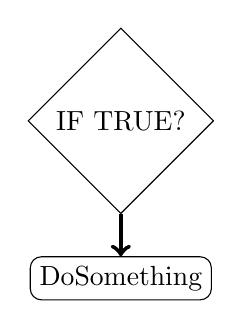
\begin{tikzpicture}[node distance=2cm]
			\node (if) [boxif] {IF TRUE?};
			\node (true) [squared,below of=if] {DoSomething};
			%-----------------------------------------------
			%-----------------------------------------------
			\draw [connect] (if) -- (true);
			\end{tikzpicture}
			\caption{Diagram if}
		\end{center}
	\end{figure}
	Contoh:
	\begin{minted}[frame=lines,fontsize=\footnotesize]{c}
unsigned char a=5;
if(a==5){
	printf("benar\n");
}
	\end{minted}
	
	\subsubsection{if-else}
	if-else mengecek suatu statement di sebelah if.
	Jika benar, statement yang sesuai dijalankan,
	Jika tidak, jalan pilihan satunya.
	\begin{minted}[frame=lines,fontsize=\footnotesize]{c}
if(kondisi){
	statement;
}
else{
	statement;
}
	\end{minted}
	Secara diagram.
	
		\begin{figure}[H]
		\begin{center}
			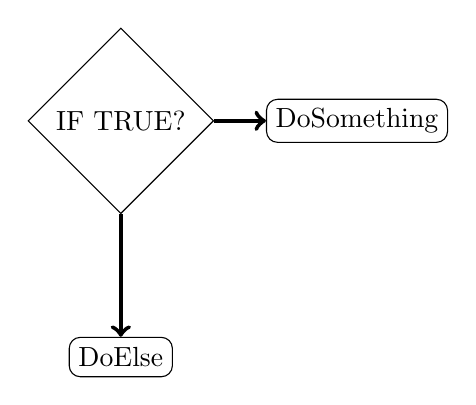
\begin{tikzpicture}[node distance=3cm]
			\node (if) [boxif] {IF TRUE?};
			\node (false) [squared,below of=if] {DoElse};
			\node (true) [squared,right of=if] {DoSomething};
			%-----------------------------------------------
			%-----------------------------------------------
			\draw [connect] (if) -- (true);
			\draw [connect] (if) -- (false);
			\end{tikzpicture}
			\caption{Diagram if-else}
		\end{center}
	\end{figure}
	Contoh:
	\begin{minted}[frame=lines,fontsize=\footnotesize]{c}
unsigned char a=5;
if(a==5){
	printf("benar\n");
}
else{
	printf("salah\n");	
}
	\end{minted}
	
	\subsubsection{if-elseif-else}
	Decision ini sama dengan if-else, namun memiliki pilihan/kemungkinan lebih dari 2.
\begin{minted}[frame=lines,fontsize=\footnotesize]{c}
if(kondisi){
	statement;
}
else if(kondisi){
	statement;
}
else{
	statement;
}
\end{minted}
	Secara diagram.
	
	\begin{figure}[H]
		\begin{center}
			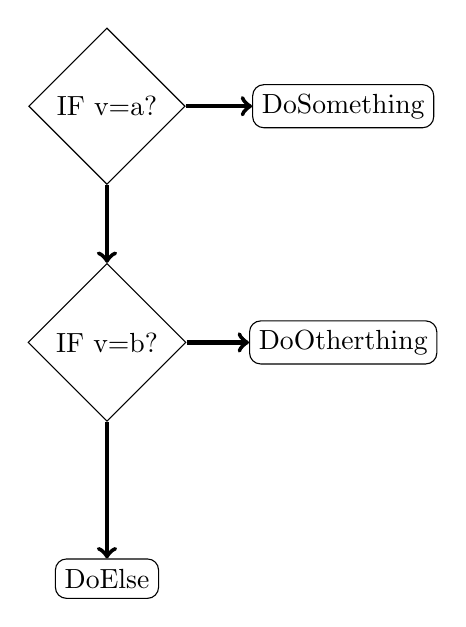
\begin{tikzpicture}[node distance=3cm]
			\node (ifa) [boxif] {IF v=a?};
			\node (ifb) [boxif,below of=ifa] {IF v=b?};
			\node (truea) [squared,right of=ifa] {DoSomething};
			\node (trueb) [squared,right of=ifb] {DoOtherthing};
			\node (false) [squared,below of=ifb] {DoElse};
			%-----------------------------------------------
			%-----------------------------------------------
			\draw [connect] (ifa) -- (truea);
			\draw [connect] (ifa) -- (ifb);
			\draw [connect] (ifb) -- (trueb);
			\draw [connect] (ifb) -- (false);
			\end{tikzpicture}
			\caption{Diagram if-elseif-else}
		\end{center}
	\end{figure}
	Contoh:
	\begin{minted}[frame=lines,fontsize=\footnotesize]{c}
unsigned char a=5;
if(a==5){
	printf("benar\n");
}
else if(a==4){
	printf("kurang\n");	
}
else{
	printf("salah\n");
}
	\end{minted}
	
	\subsubsection{switch-case}
	Decision ini khhusus jika yang dicek adalah variabel, bukan statement, fungsi, atau operasi.
	\begin{minted}[frame=lines,fontsize=\footnotesize]{c}
switch(a){
	case 1: statement; break;
	case 2: statement; break;
	case 3: statement; break;
	default: statement;
	
}
	\end{minted}
	
	Secara diagram.
	
	\begin{figure}[H]
		\begin{center}
			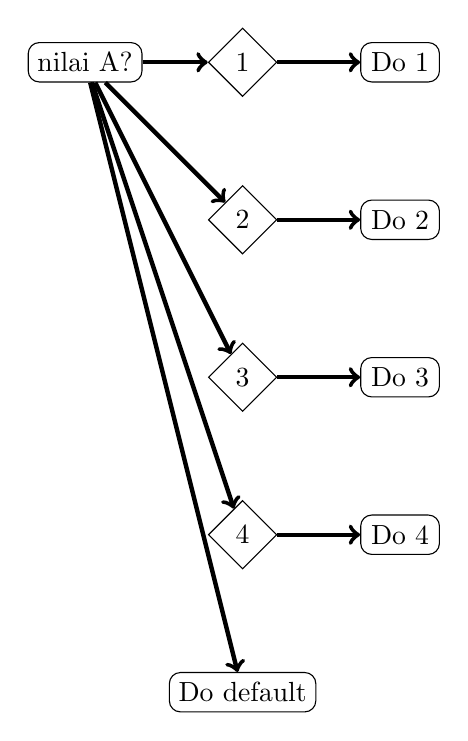
\begin{tikzpicture}[node distance=2cm]
			\node (if) [squared] {nilai A?};
			\node (if1) [boxif,right of=if] {1};
			\node (if2) [boxif,below of=if1] {2};
			\node (if3) [boxif,below of=if2] {3};
			\node (if4) [boxif,below of=if3] {4};
			\node (ifnone) [squared,below of=if4] {Do default};
			\node (ok1) [squared,right of=if1] {Do 1};
			\node (ok2) [squared,right of=if2] {Do 2};
			\node (ok3) [squared,right of=if3] {Do 3};
			\node (ok4) [squared,right of=if4] {Do 4};
			
			\draw [connect] (if) -- (if1);
			\draw [connect] (if) -- (if2);
			\draw [connect] (if) -- (if3);
			\draw [connect] (if) -- (if4);
			\draw [connect] (if) -- (ifnone);
			\draw [connect] (if1) -- (ok1);
			\draw [connect] (if2) -- (ok2);
			\draw [connect] (if3) -- (ok3);
			\draw [connect] (if4) -- (ok4);

			\end{tikzpicture}
			\caption{Diagram switch-case}
		\end{center}
	\end{figure}
	Contoh:
	\begin{minted}[frame=lines,fontsize=\footnotesize]{c}
unsigned char a;
siwtch(a){
	case 1: 
		do_A();
		break;
	case 2:
		do_B();
		break;
	case 3: 
		do_C();
		break;
	case 4: 
		do_D();
		break;
	default:
		do_default();
}
	\end{minted}
	
	\newpage
	\subsection{Loop}
	
	Loop ada bagian bahasa pemrograman yang berguna untuk mengulang statemen.
	
	\subsubsection{for}
	for untuk mengulang statemnet dalam jumlah yang sudah ditentukan.
	Pola nya:
\begin{minted}[frame=lines,fontsize=\footnotesize]{c}
for(nilai_awal;batas_akhir;perubahan_tiap_loop){
	statement;
}
\end{minted}
	Secara diagram.
	
	\begin{figure}[H]
		\begin{center}
			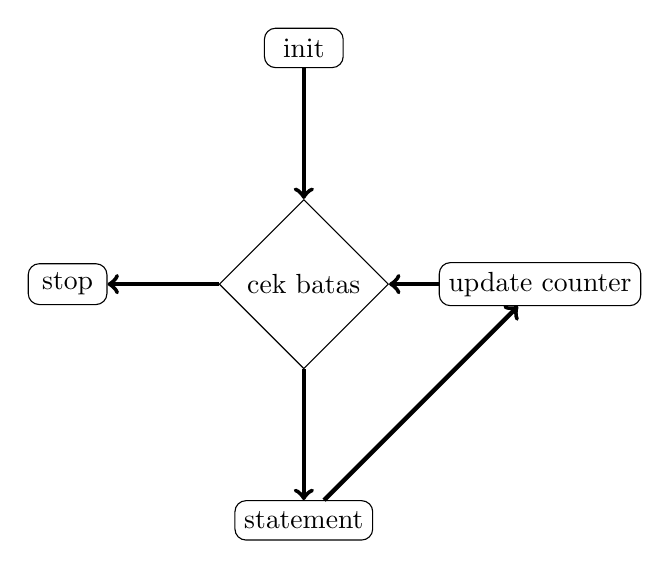
\begin{tikzpicture}[node distance=3cm]
			\node (init) [squared] {init};
			\node (batas) [boxif,below of=init] {cek batas};
			\node (cnt) [squared,right of=batas] {update counter};
			\node (state) [squared,below of=batas] {statement};
			\node (stop) [squared,left of=batas] {stop};

			\draw [connect] (init) -- (batas);
			\draw [connect] (batas) -- (state);
			\draw [connect] (state) -- (cnt);
			\draw [connect] (cnt) -- (batas);
			\draw [connect] (batas) -- (stop);
			\end{tikzpicture}
			\caption{Diagram loop for}
		\end{center}
	\end{figure}
	Contoh:
	\begin{minted}[frame=lines,fontsize=\footnotesize]{c}
unsigned char i;
for(i=0;i<10;i++){
	printf("loop\n");
}
	\end{minted}
		
	\subsubsection{while}
	while untuk untuk mengulang statemnet selama kondisi sesuai.
	Jika menggunakan variabel, maka harus ada update nilai dalam loop
	Pola nya:
	\begin{minted}[frame=lines,fontsize=\footnotesize]{c}
while(kondisi){
	statement;
}
	\end{minted}
	Secara diagram.
	
	\begin{figure}[H]
		\begin{center}
			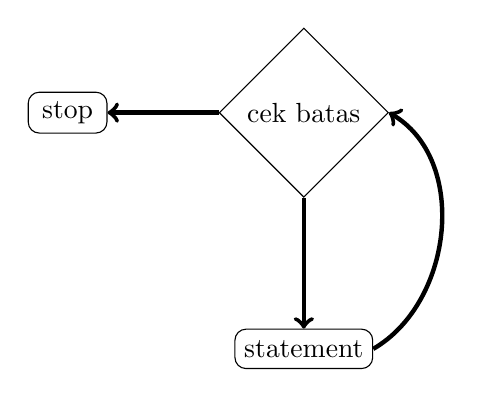
\begin{tikzpicture}[node distance=3cm]
			\node (batas) [boxif] {cek batas};
			\node (state) [squared,below of=batas] {statement};
			\node (stop) [squared,left of=batas] {stop};
			
			\draw [connect] (batas) -- (state);
			\draw [connect] (state.east) to [out=30,in=330] (batas.east);
			\draw [connect] (batas) -- (stop);
			\end{tikzpicture}
			\caption{Diagram loop while}
		\end{center}
	\end{figure}
	Contoh:
	\begin{minted}[frame=lines,fontsize=\footnotesize]{c}
unsigned char i;
while(i<10){
	printf("loop\n");
	i++;
}
	\end{minted}
	
	\subsubsection{do-while}
	do-while untuk sama dengan while, bedanya check batas diakhir, sehingga minimal loop jalan 1x..
	Jika menggunakan variabel, maka harus ada update nilai dalam loop
	Pola nya:
	\begin{minted}[frame=lines,fontsize=\footnotesize]{c}
do{
	statement;
}while(kondisi);
	\end{minted}
	Secara diagram.
	
	\begin{figure}[H]
		\begin{center}
			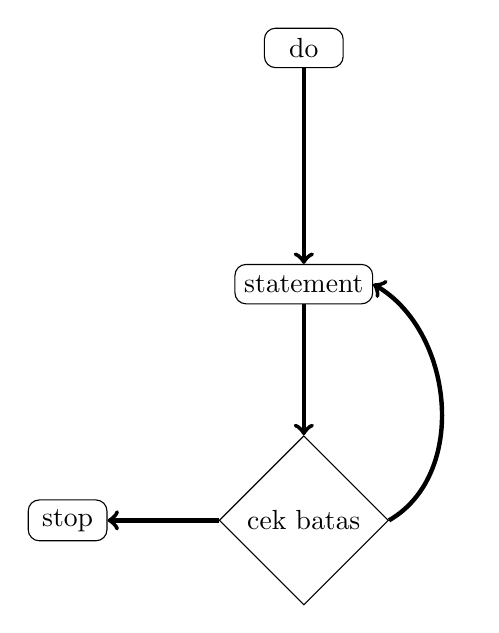
\begin{tikzpicture}[node distance=3cm]
			\node (do) [squared] {do};
			\node (state) [squared,below of=do] {statement};
			\node (batas) [boxif,below of=state] {cek batas};
			\node (stop) [squared,left of=batas] {stop};
			
			\draw [connect] (do) -- (state);
			\draw [connect] (state) -- (batas);
			\draw [connect] (batas.east) to [out=30,in=330] (state.east);
			\draw [connect] (batas) -- (stop);
			\end{tikzpicture}
			\caption{Diagram loop while}
		\end{center}
	\end{figure}
	Contoh:
	\begin{minted}[frame=lines,fontsize=\footnotesize]{c}
unsigned char i;
do{
	print("loop\n");
	i++;
}while(i<10);

	\end{minted}
	
	\newpage
	\subsection{Fungsi}
	
	Fungsi adalah sekumpulan statemen yang bersinergi untuk tugas tertentu.
	Fungsi dapat mengambil satu atau lebih variabel input.
	Fungsi hanya dapat menghasilkan satu atau kosong variable output.
	
	\subsubsection{Bentuk}
	Bentuk umum Fungsi adalah sebagai berikut:
	\begin{minted}[frame=lines,fontsize=\footnotesize]{c}
<type_out> nama_fungsi(<type_in> variable_input){
	<type_out> variabel_output;
	statement;
	return variabel_output;
}
	\end{minted}
	Penjelasan:
	\begin{itemize}
		\item \textbf{<type\_out>} adalah penanda jenis tipe data variabel keluaran.
		Pilihan <type\_out> sama dengan tipe data untuk variabel (char, int, float, dst).
		Selain tipe data, <type\_out> juga dapat berupa \textbf{void}.
		Fungsi <type\_out> void artinya adalah fungsi yang berjalan tanpa mengeluarkan output.
		
		\item \textbf{nama\_fungsi} adalah nama untuk fungsi itu sendiri.
		Aturan penamaan fungsi sama dengan aturan penamaan variabel.
		
		\item \textbf{<type\_in>} adalah penanda jenis tipe data variabel masukan.
		Pilihan <type\_in> sama dengan tipe data untuk variabel (char, int, float, dst).
		
		\item \textbf{variable\_input} adalah variabel untuk input fungsi itu sendiri.
		
		\item \textbf{variable\_output} adalah variabel yang diawali statement \textbf{return} agar mengeluarkan hasil fungsi.
		tipe data variable\_output harus sama dengan <type\_out>.
	\end{itemize}

	Berikut beberapa contoh fungsi:
	\begin{itemize}
		\item Fungsi dengan input-output
		\begin{minted}[frame=lines,fontsize=\footnotesize]{c}
char jumlah(char A, char B){
	char C;
	C = A + B;
	return C;
}
		\end{minted}
		
		\item Fungsi dengan input tanpa output.
		Fungsi seperti ini pada umumnya memanipulasi variabel global.
		\begin{minted}[frame=lines,fontsize=\footnotesize]{c}
void jumlah(char A, char B){
	char C;
	C = A + B;
}
		\end{minted}
		
		\item Fungsi dengan output tanpa input
		\begin{minted}[frame=lines,fontsize=\footnotesize]{c}
char jumlah(void){
	char C;
	C = 1 + 2;
	return C;
}
		\end{minted}
		
		\item Fungsi dengan tanpa input-output.
		Fungsi seperti ini pada umumnya memanipulasi variabel global.
		\begin{minted}[frame=lines,fontsize=\footnotesize]{c}
unsigned char A,B,C;
void jumlah(void){
	C = B + C;
}
		\end{minted}
		
	\end{itemize}
	
	\subsubsection{Main}
	
	Dalam pemrograman bahasa C, ada satu nama fungsi yang khusus dimana fungsi ini menjadi fungsi yang paling pertama dijalankan.
	Fungsi tersebut disebut fungsi \textbf{main}.
	Setiap project atau kode sumber dalam bahasa C/C++, wajib ada 1 dan hanya 1 fungsi main.
	Secara umum bentuknya:
	
	\begin{minted}[frame=lines,fontsize=\footnotesize]{c}
int main(void){
	statement;
	return 0
}
	\end{minted}
	
	\subsubsection{Prototype}
	
	Konsep \textit{Prototype} adalah pemisahan antara deklarasi fungsi dan referensi fungsi.
	Berikut dijelaskan konsep tersebut dengan contoh.
	
	Suatu fungsi diklarasikan sebelum fungsi \textbf{main()}.
	\begin{minted}[frame=lines,fontsize=\footnotesize]{c}
int jumlah(int X, int Y);
	\end{minted}
	
	Pada bagian ini, fungsi masih berupa deklarasi prototype namun sudah dapat dipanggil oleh fungsi lain.
	Sebagai contoh dipanggil di fungsi main():
	\begin{minted}[frame=lines,fontsize=\footnotesize]{c}
int main(){
	int A,B,C;
	A=B=5;
	C=jumlah(A,B);
	return 0;
}
	\end{minted}
	
	Pada tahapan ini, kode sumber dapat di kompile namun akan error dan protes meminta referensi dari fungsi yang telah di prototype.
	Maka di suatu tempat di kode sumber setelah main(), perlu dibuat referensi fungsinya.
	Misal:
	\begin{minted}[frame=lines,fontsize=\footnotesize]{c}
int jumlah(int X, int Y){
	int Z;
	Z=X+Y;
	return Z;
}
	\end{minted}
	
	Pada tahapan ini, lengkap sudah fungsi tersebut baik pada prototype maupun referensi.
	
	Tambahan, sebagai pengenalan, berdasarkan deklarasi dan penggunan, dalam fungsi dikenal 2 jenis parameter input:
	\begin{itemize}
		\item Parameter Formal. Yaitu parameter yang ada saat deklarasi/referensi.
		Dalam contoh ini adalah variabel X dan Y.
		
		\item Parameter Actual. Yaitu parameter yang ada saat fungsi tersebut dipanggil atau dipakai.
		Dalam contoh ini adalah variabel A dan B.
	\end{itemize}

	Kedua jenis parameter ini dalam konsep fungsi harus memiliki tipe data yang sama.
	
	\subsubsection{Scope}
	
	Dalam pemrograman C, terdapat pemisahan hak akses variabel yang dikenal dengan istilah \textit{scope} atau cakupan.
	Terdapat dua jenis, yaitu:
	\begin{itemize}
		\item Global. Variabel jenis ini dideklarasikan di luar fungsi mana pun, sehingga dapat diakses oleh semua fungsi.
		\item Local. Variabel jenis ini dideklarasikan di dalam suatu fungsi, sehingga hanya dapat diakses selain fungsi itu sendiri.
	\end{itemize}
	 Berikut contoh:
	 \begin{minted}[frame=lines,fontsize=\footnotesize]{c}
int gA=5;

int mFungsi(void){
	int mA=10;
	return mA+gA;
}

int vFungsi(void){
	int vA=8;
	return mA+vA;
}
	 \end{minted}
	 
	 Dari contoh ini, dapat dilihat bahwa:
	 \begin{itemize}
	 	\item variabel gA adalah variabel Global.
	 	Variabel gA dapat diakses oleh mFungsi dan vFungsi.
	 	
	 	\item variabel mA adalah variabel lokal milik mFungsi.
	 	Variabel mA tidak dapat diakses vFungsi.
	 	
	 	\item variabel vA adalah variabel lokal milik vFungsi.
	 	Variabel vA tidak dapat diakses mFungsi.
	 \end{itemize}
 
 	Tips: Sebaiknya gunakan variabel global seperlunya dan seminimal mungkin.
 	Penggunaan terlalu banyak variabel global seringkali membingungkan diri sendiri.
	
	\newpage
	\subsection{Array}
	
	Array adalah gabungan banyak variabel yang memiliki nama sama dan tipe data sama, namun dibedakan oleh index/atau elemen.
	Array dalam memory selalu memiliki alamat yg berdekatan dan berurutan.
	Array selalu dihitung dari 0, sehingga jika dideklarasi array dengan jumlah index 5, maka nomor index adalah 0 sampai 4.
	Contoh deklarasi array
\begin{minted}[frame=lines,fontsize=\footnotesize]{c}
int marks[5];
\end{minted}
	Saat deklarasi, dapat juga langsung diisi nilai awal setiap index.
	Cukup ditulis semua nilai diapit kurung kurawal dan dipisah koma.
	Contoh:
\begin{minted}[frame=lines,fontsize=\footnotesize]{c}
int marks[5]={80,70,60,85,75};
\end{minted}
	atau jika dengan menulis anggota, tidak perlu mengisi nilai total index.
	\begin{minted}[frame=lines,fontsize=\footnotesize]{c}
int marks[]={80,70,60,85,75};
	\end{minted}
	
	Berikut contoh variabel array \textbf{marks} dengan jumlah index 5.
	
	\begin{figure}[H]
		\centering
		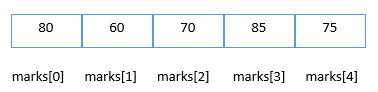
\includegraphics[width=0.35\linewidth]{images/array}
		\caption{contoh gambaran Array}
	\end{figure}
	
	\subsubsection{Akses Array}
	
	Untuk akses Array, sama dengan variabel pada umumnya, hanya saya wajib menyertakan pada index ke berapa variabel yang diakses.
	Contoh memanggil nilai dari array:
	\begin{minted}[frame=lines,fontsize=\footnotesize]{c}
int A=marks[1];
	\end{minted}
	
	Contoh mengisi nilai array:
	\begin{minted}[frame=lines,fontsize=\footnotesize]{c}
marks[1]=12;
	\end{minted}
	
	Salah satu keuntungan array adalah akses dapat berupa variabel.
	Contoh untuk looping:
	\begin{minted}[frame=lines,fontsize=\footnotesize]{c}
for(i=0;i<5;i++){
	marks[i]=0;
}
	\end{minted}
	
	\subsubsection{String}
	
	Variabel bertipe char dapat digunakan untuk menyimpan satu digit teks (huruf atau angka) dalam standar ASCII.
	Angka atau huruf dimasukan dengan diapit petik 1 (').
	Sebagai contoh:
	\begin{minted}[frame=lines,fontsize=\footnotesize]{c}
char A='A';
char dua='2';
	\end{minted}
	
	Untuk membentuk kata, bisa digunakan array khusus yang dikenal sebagai \textbf{string}.
	String adalah array yang berisi teks (huruf atau angka).
	String selalu diakhiri karaketer \textbf{null} ('\textbackslash0').
	Berikut contohnya:
	\begin{minted}[frame=lines,fontsize=\footnotesize]{c}
char kata[]={'s','a','y','a','\0'};
	\end{minted}
	
	Atau dengan cara yang lebih familiar, yaitu menggunakan tanda petik dobel (").
	Jika memilih cara ini, tidak diakhiri karaketer \textbf{null} dan kurung kurawal.
	\begin{minted}[frame=lines,fontsize=\footnotesize]{c}
char kata[]="saya";
	\end{minted}
	
	\subsubsection{Fungsi manipulasi string}
	Berikut beberapa fungsi untuk manipulasi string:
	\begin{itemize}
		\item sprintf(). Untuk mengisi suatu array dengan data teks tidak saat deklarasi array.
		Contoh:
		\begin{minted}[frame=lines,fontsize=\footnotesize]{c}
char teks[10];
sprintf(teks,"saya");
		\end{minted}
		
		\item strcpy(), untuk mengisi satu string dengan variabel string lain.
		\begin{minted}[frame=lines,fontsize=\footnotesize]{c}
strcpy(string_tujuan, string_asal);
		\end{minted}
		
		\item strcat(), untuk menyambungkan dua string.
		\begin{minted}[frame=lines,fontsize=\footnotesize]{c}
strcat(string_tujuan, string_tambahan);
		\end{minted}
		
		\item strlen(), untuk mengetahui panjang suatu string.
		\begin{minted}[frame=lines,fontsize=\footnotesize]{c}
int lkata=strlen(kata);
		\end{minted}
		
		\item strcmp(), untuk komparasi 2 string.
		Akan menghasilkan nilai 0 jika kedua string sama.
		\begin{minted}[frame=lines,fontsize=\footnotesize]{c}
int vStr=strcmp(s1,s2);
		\end{minted}
	\end{itemize}
	
	\newpage
	\subsection{Input-Output}
	Input-Output yang akan dijelaskan adalah metode yang banya digunakan untuk mengambil input dan menghasilkan output dalam bentuk variabel.
		
	\subsubsection{Format specifiers}
	Dalam penggunaan teks input-output, diperlukan jenis string pengganti dalam sebuah kata yang bersesuaian dengan type data variabel yang digunakan.
	String ini dikenal sebagai Format specifiers.
	Bentuk umumnya adalah tanda persen \% diikuti specifier yang sesuai.
	Berikut tabelnya:
	
	\begin{table}[H]
		\begin{tabular}{|l|l|l}
			\cline{1-2}
			\textbf{specifier} & \textbf{type-data} \\ \cline{1-2}
			\%i & char, integer \\ \cline{1-2}
			\%x & char, integer (hexa) \\ \cline{1-2}
			\%f & float \\ \cline{1-2}
			\%d & doubel \\ \cline{1-2}
			\%c & character (ASCII) \\ \cline{1-2}
			\%s & string \\ \cline{1-2}
		\end{tabular}
	\end{table}

	Format spesifier dapat pula ditentukan ukuran digitnya, dengan menaruh angka antara \% dan huruf specifier. 
	Contoh
	\begin{minted}[frame=lines,fontsize=\footnotesize]{c}
unsigned int A=5;	
printf("nilai = %i",A); // hasilnya "nilai = 5"
printf("nilai = %5i",A); // hasilnya "nilai =     5"
	\end{minted}
	
	Khusus \%f dan \%d, kita bisa mengatur jumlah angka dibelakang koma, juga dengan menaruh angka antara \% dan huruf specifier.
	Namun angka memilki pola X.Y, dimana X adalah total ukuran dan Y adalah jumlah angka dibelakang koma.
	Sisa angka depan koma dihitung dengan X-(Y+1).
	Nilai Y ditambah 1 karena koma juga dihitung memiliki space.
	Jika angka dibelakang koma lebih banyak daripada space yang ada, maka otomatis dibulatkan.
	Contoh
	\begin{minted}[frame=lines,fontsize=\footnotesize]{c}
float A=45.236;	
printf("nilai = %5.2i",A); // hasilnya "nilai = 45.24"
	\end{minted}
	
	\subsubsection{printf}
	
	Fungsi printf() digunakan untuk menampilkan teks dengan menggunakan format specifier.
	Agar rapi, seringkali printf() dalam argumennya diakhiri "\textbackslash r\textbackslash n".
	Pola umum:
	\begin{minted}[frame=lines,fontsize=\footnotesize]{c}
printf("teks");
printf("teks dengan specifier",v1,v2,v3);
printf(variabel_string);
	\end{minted}
	
	Berikut beberapa contoh:
	\begin{itemize}
		\item Tampilkan kata/kalimat saja
		\begin{minted}[frame=lines,fontsize=\footnotesize]{c}
printf("Hellowww \n\r");
		\end{minted}
		
		\item Tampilkan variabel berisi nilai integer
		\begin{minted}[frame=lines,fontsize=\footnotesize]{c}
unsigned int vA=10;
unsigned int vB=11;
printf("nilai vA= %i dan vB = %i \n\r",vA,vB);
		\end{minted}
		
		\item Tampilkan variabel berisi string
		\begin{minted}[frame=lines,fontsize=\footnotesize]{c}
char test[]="seloww \n\r";
printf(test);
		\end{minted}
		
		\item Tampilkan variabel berisi string dengan format specifier
		\begin{minted}[frame=lines,fontsize=\footnotesize]{c}
char test[]="seloww";
printf("isi test %s \n\r",test);
		\end{minted}
	\end{itemize}

	\subsubsection{scanf}
	
	Fungsi scanf() adalah kebalikan dan printf, yaitu membaca input teks/string.
	Hasil pembacaan akan dimasukkan ke dalam variabel string atau array char.
	Pembacan dianggap selesai jika ada input Return atau Enter.
	Pola umum:
	\begin{minted}[frame=lines,fontsize=\footnotesize]{c}
char variabel_tujuan[max_char];

scanf("%s",variabel_tujuan);
	\end{minted}
	
	Contoh penggunaan scanf():
	\begin{minted}[frame=lines,fontsize=\footnotesize]{c}
char teks_in[10];
scanf("%s",teks_in);
printf(teks);
	\end{minted}
	
	\subsubsection{Konversi String}
	
	Dalam penggunaan scanf(), hasil akhir pembacaan selalu sebagai string.
	Apabila jika input yang diinginkan adalah angka/nilai yang dapat dioperasikan, maka perlu dikonversi.
	Fungsi-fungsi konversi tersedia di pustaka \textbf{stdlib} sehingga perlu inklusi:
	\begin{minted}[frame=lines,fontsize=\footnotesize]{c}
#include <stdlib.h>
	\end{minted}
	
	Berikut fungsi konversi yang sering digunakan:
	\begin{itemize}
		\item String-Integer. Fungsi yang digunakan adalah \textbf{atoi()}.
		\begin{minted}[frame=lines,fontsize=\footnotesize]{c}
char text_in[10];
unsigned int num;

scanf("%s",text_in);
num=atoi(text_in);
printf("num= %i",num);
		\end{minted}
		
		\item String-Float. Fungsi yang digunakan adalah \textbf{atof()}.
		Perlu diperhatikan, saat input bilangan dengan koma, pemisah decimal adalah titik (.) bukan koma (,).
		\begin{minted}[frame=lines,fontsize=\footnotesize]{c}
char text_in[10];
float num;

scanf("%s",text_in);
num=atof(text_in);
printf("num= %5.2f",num);
		\end{minted}
	
	\end{itemize}

	\subsubsection{Karakter Escape}
	Dalam penggunaan printf()/scanf(), terdapat karakter khusus yang memiliki kegunaan tertentu.
	Karakter ini disebut \textbf{Escape Character}.
	Berikut yang sering digunakan:
	\begin{table}[H]
		\begin{tabular}{|l|l|l|l}
			\cline{1-3}
			\textbf{character} & \textbf{nama} & \textbf{arti} \\ \cline{1-3}
			\textbackslash n          & Line Feed	   & Memberikan garis baru        \\ \cline{1-3}
			\textbackslash r          & Carriage Return & Menyebab baris ke tepi kiri  \\ \cline{1-3}
			\textbackslash \textbackslash & Backslash       & Menyebab karaketer Backslash \\ \cline{1-3}
			\textbackslash t          & Horizontal Tab  & Menyebab Tab mendatar        \\ \cline{1-3}
			\textbackslash v          & Vertical Tab    & Menyebab Tab vertikal        \\ \cline{1-3}
			\textbackslash '          & Single Quote    & Menyebab petik satu          \\ \cline{1-3}
			\textbackslash "          & Double Quotes   & Menyebab petik dua           \\ \cline{1-3}
			\textbackslash ?          & Question Mark   & Menyebab tanda tanya         \\ \cline{1-3}
		\end{tabular}
	\end{table}
	
	\newpage
	\subsection{Preprocessor}
	
	Preprocessor adalah statement yang akan dilakukan sebelum proses kompilasi lebih lanjut.
	Preprocessor membantu proses kompilasi menjadi lebih terarah sesuai kebutuhan, namun tidak secara langsung memanipulasi program akhir.
	
	Beberapa Preprocessor yang sering digunakan antara lain:
	\begin{itemize}
		\item \textbf{\#include}. \\
		Preprocessor ini digunakan untuk inklusi (mengikutkan) suatu file header.
		Contoh untuk header yang dimiliki kompiler.
		\begin{minted}[frame=lines,fontsize=\footnotesize]{c}
#include <stdio.h>
		\end{minted}
		
		Contoh untuk header yang dibuat sendiri.
		Perbedaanya adalah tanda (< >) diganti (" ").
		\begin{minted}[frame=lines,fontsize=\footnotesize]{c}
#include "alcd"
		\end{minted}
		
		\item \textbf{\#define}. \\
		Preprocessor ini digunakan untuk mendefinisikan suatu macro secara global.
		Macro adalah suatu statement yang dilihat kompiler namun tidak termasuk kode sumber yang membangun binary.
		Preprocessor ini sering digunakan untuk identifikasi konstanta.
		Contoh.
		\begin{minted}[frame=lines,fontsize=\footnotesize]{c}
#define PI 3.14
		\end{minted}
		dengan definisi ini, maka setiap ada statement PI akan dibaca sebagai 3.14.
		Defini preprocessor ini juga dapat digunakan dalam bentuk definisi global tanpa nilai tertentu.
		Contoh:
		\begin{minted}[frame=lines,fontsize=\footnotesize]{c}
#define USE_SYSTEM
		\end{minted}
		
		\item \textbf{\#undef}. \\
		Kebalikan \#define, yaitu menghapus suatu definisi macro.
		
		\item \#ifdef atau \#ifndef, \#else, dan \#endif. \\
		Bersama dengan \#define, preprocessor ini digunakan sebagai pengaturan statemen mana yang akan dikompilasi.
		Penggunaannya mirip dengan decision if-else namun nilai benarnya adalah ketika suatu definisi telah didefinisikan.
		Contoh:
		\begin{minted}[frame=lines,fontsize=\footnotesize]{c}
#define USE_SYSTEM
#ifdef USE_SYSTEM
	void nilai(int vA);
#else
	void nilai(int vA,int vB);
#endif
		\end{minted}
		Dalam contoh ini, yang dilihat kompiler adalah prototype fungsi dengan satu argumen.
		
		\item \textbf{\#ifndef}, \textbf{\#else}, dan \textbf{\#endif}. \\
		Sama seperti sebelumnya, namun kondisi yang dicari sebaliknya yaitu benar jika suatu definisi tidak terdefinisi
		Contoh:
		\begin{minted}[frame=lines,fontsize=\footnotesize]{c}
#ifndef USE_SYSTEM
	#define USE_SYSTEM
#endif
		\end{minted}
		Dalam contoh ini, yang akan didefinisikan USE\_SYSTEM jika belum didefinisikan.
		
		\item \textbf{\#if}, \textbf{\#else}, dan \textbf{\#endif}. \\
		Persis sama dengan decision if-else, namun dalam skala preprocessor dan kondisi yang terdefinisi 1 atau 0.
		Contoh:
		\begin{minted}[frame=lines,fontsize=\footnotesize]{c}
#define USE_SYSTEM 1
#if USE_SYSTEM
	void nilai(int vA);
#else
	void nilai(int vA,int vB);
#endif
		\end{minted}
		Dalam contoh ini, yang dilihat kompiler adalah prototype fungsi dengan satu argumen.
		
	\end{itemize}
	
	
	\newpage
	\subsection{Header-Multisources}
	
	Pada bagian ini, akan dikenalkan metode pemrograman dengan memisahkan file-file berdasarkan kebutuhan.
	Disini akan dicoba memisahkan kode sumber dalam 2 file dengan dijembatani 1 file header.
	
	File header adalah file berekstensi *.h yang berisi inklusi pustaka yang dibutuhkan, defisini macro, dan deklarasi prototype fungsi.
	Nama file header umumnya sama dengan nama file source yang berasosiasi dan menjadi jembatan pengenal untuk source tersebut.
	Untuk memudahkan, lakukan langkah berikut:
	\begin{enumerate}
		\item tambahkan satu lagi file C source dengan nama \textbf{jumlah.c}.
		Jangan lupa centang \textbf{all} untuk menambahkan file ke build target.
		\begin{figure}[H]
			\centering
			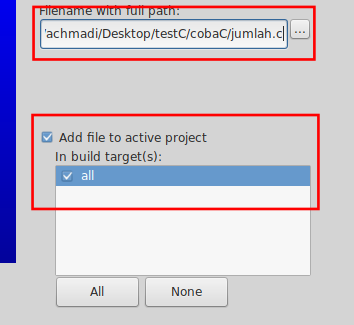
\includegraphics[width=0.35\linewidth]{images/c_mul_0}
			\caption{tambahkan satu lagi source}
		\end{figure}
	
		\item file header baru.
		\begin{figure}[H]
			\centering
			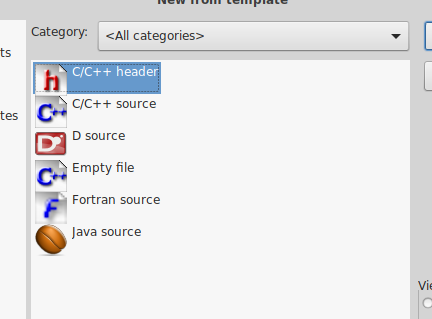
\includegraphics[width=0.35\linewidth]{images/c_mul_1}
			\caption{buat header baru}
		\end{figure}
	
		\item tambahkan 1 file header dengan nama \textbf{jumlah.h}
		Jangan lupa centang \textbf{all} untuk menambahkan file ke build target.
		\begin{figure}[H]
			\centering
			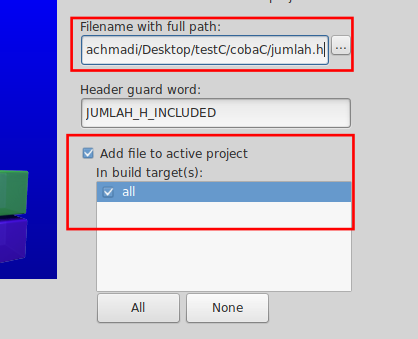
\includegraphics[width=0.35\linewidth]{images/c_mul_2}
			\caption{tambahkan satu file header}
		\end{figure}
	
		\item hasil semmua file tambahan (jumlah.c dan jumlah.h).
		\begin{figure}[H]
			\centering
			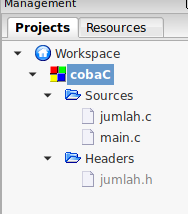
\includegraphics[width=0.35\linewidth]{images/c_mul_3}
			\caption{hasil}
		\end{figure}
	
		\item pastikan semua sudah masuk ke build target.
		Klik menu \textbf{Properties} -> tab \textbf{Build Targets}.
		\begin{figure}[H]
			\centering
			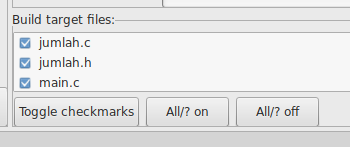
\includegraphics[width=0.35\linewidth]{images/c_mul_4}
			\caption{build target}
		\end{figure}
	\end{enumerate}

	Selanjutnya isi setiap file sebagai berikut:
	\begin{itemize}
		\item jumlah.h
		\begin{minted}[frame=lines,fontsize=\footnotesize]{c}
#ifndef JUMLAH_H_INCLUDED
#define JUMLAH_H_INCLUDED

#include <stdio.h>

#define KONS 100

unsigne int jumlah(unsigned int vA);

#endif
		\end{minted}
		Disini didekalarasikan beberapa entitas:
		\begin{itemize}
			\item prototype fungsi jumlah()
			\item macro KONS yang akan dibaca kompiler sebagai nilai 100
		\end{itemize}
		 
		
		\item jumlah.c
		\begin{minted}[frame=lines,fontsize=\footnotesize]{c}
#include "jumlah.h"

unsigned int vCons = 25;

unsigned int jumlah(unsigned int vA){
	return vA + KONS;
}
		\end{minted}
		Disini secara pokok berisi:
		\begin{itemize}
			\item inklusi jumlah.h
			\item deklarasi variabel global vCons.
			\item referensi fungsi jumlah()
		\end{itemize}
	
		\item main.c
		\begin{minted}[frame=lines,fontsize=\footnotesize]{c}
#include <stdio.h>
#include "jumlah.h"

extern unsigned int vCons;

int main() {
	unsigned int vX,vY;
	vX=2*vCons;
	vY=jumlah(vX);
	vY+=KONS;
	printf("nilai akhir %i",vY);
	return 0;
}

		\end{minted}
		
		Disini secara pokok berisi:
		\begin{itemize}
			\item inklusi jumlah.h
			\item deklarasi ulang variabel global vCons.
			Disini penanda \textbf{extern} digunakan dan tidak diisi nilai awal, karena deklarasi yang sebenarnya ada di file jumlah.c.
			\item fungsi main()
			\item penggunaan fungsi jumlah() dan macro KONS.
		\end{itemize}
	\end{itemize}

	\newpage
	\subsection{Rangkuman}
	
	\subsubsection{Hello World}
	\begin{minted}[frame=lines,fontsize=\footnotesize]{c}
#include <stdio.h>

int main() {
	printf("hello world);
	return 0;
}
	\end{minted}
	
	\subsubsection{Komentar}
	\begin{minted}[frame=lines,fontsize=\footnotesize]{c}
// contoh komentar
unsigned int vt=0; //sebelah ini bukan komentar
// per baris

/* contoh komentar
unsigned int vt=0; (sebelah ini ikut jadi komentar)
per baris */
	\end{minted}
	
	\subsubsection{Deklarasi Variabel}
	\begin{minted}[frame=lines,fontsize=\footnotesize]{c}
unsigned char v_8bit; //0 255
char v_8bit; //(-+) 128

unsigned int v_16bit; //0 65,535
int v_16bit; //(-+)32,778

unsigned long v_32bit; //0 4,294,967,295
long v_32bit; //(-+)2,147,483,647

float v_dec; //32bit decimal

double v_64bit; //64bit decimal
	\end{minted}
	
	\subsubsection{TypeCast}
	\begin{minted}[frame=lines,fontsize=\footnotesize]{c}
unsigned char a,b;
unsigned int c;

a=b=250;
c=(unsigned int)a+b;
	\end{minted}
	
	\subsubsection{Penulisan Konstanta}
	\begin{table}[H]
		\begin{tabular}{|l|l|l|l}
			\cline{1-3}
			\textbf{decimal} & \textbf{biner} & \textbf{hexa} \\ \cline{1-3}
			0 & 0b0000 & 0x0  \\ \cline{1-3}
			1 & 0b0001 & 0x1  \\ \cline{1-3}
			2 & 0b0010 & 0x2  \\ \cline{1-3}
			3 & 0b0011 & 0x3  \\ \cline{1-3}
			4 & 0b0100 & 0x4  \\ \cline{1-3}
			5 & 0b0101 & 0x5  \\ \cline{1-3}
			6 & 0b0110 & 0x6  \\ \cline{1-3}
			7 & 0b0111 & 0x7  \\ \cline{1-3}
			8 & 0b1000 & 0x8  \\ \cline{1-3}
			9 & 0b1001 & 0x9  \\ \cline{1-3}
			10 & 0b1010 & 0xA  \\ \cline{1-3}
			11 & 0b1011 & 0xB  \\ \cline{1-3}
			12 & 0b1100 & 0xC  \\ \cline{1-3}
			13 & 0b1101 & 0xD  \\ \cline{1-3}
			14 & 0b1110 & 0xE  \\ \cline{1-3}
			15 & 0b1111 & 0xF  \\ \cline{1-3}
		\end{tabular}
	\end{table}

	\subsubsection{Operator}
	\begin{minted}[frame=lines,fontsize=\footnotesize]{c}
unsigned char a,b,c;

a=6;
b=2;

c=a*b; //c=12
c=a/b; //c=3
c=a+b; //c=8
c=a-b; //c=4
c=a%b; //c=0
	\end{minted}
	
	\begin{minted}[frame=lines,fontsize=\footnotesize]{c}
unsigned char a=6;

a=a+2; //nilai akhir a menjadi 8
a+=2; //sama

a+=1; //nilai akhir a menjadi 7
a++; //sama (khusus penambahan 1)
	\end{minted}
	
	\begin{minted}[frame=lines,fontsize=\footnotesize]{c}
unsigned int a,b;
a=1;
b=0;

if(a==b){printf("benar");}
if(a!=b){printf("salah");}
if(a>b) {printf("benar");}
if(a>=b){printf("benar");}
if(a<b) {printf("salah");}
if(a<=b){printf("salah");}

if(a&&b){printf("salah");}
if(a||b){printf("benar");}
if(!a)  {printf("salah");}
	\end{minted}
	
	\subsubsection{Decision}
	\begin{minted}[frame=lines,fontsize=\footnotesize]{c}
if(kondisi){
	printf("benar");
}
	\end{minted}
	
	\begin{minted}[frame=lines,fontsize=\footnotesize]{c}
if(kondisi){
	printf("benar");
}
else{
	printf("selainnya");
}
	\end{minted}
	
	\begin{minted}[frame=lines,fontsize=\footnotesize]{c}
if(kondisi){
	printf("benar satu");
}
else if {
	printf("benar dua");
}
	\end{minted}
	
	\begin{minted}[frame=lines,fontsize=\footnotesize]{c}
if(kondisi){
	printf("benar satu");
}
else if {
	printf("benar dua");
}
else{
	printf("selainnya");
}
	\end{minted}
	
	\begin{minted}[frame=lines,fontsize=\footnotesize]{c}
unsigned int A;

switch(A){
	case 1: printf("nilai 1"); break;
	case 2: printf("nilai 2"); break;
	case 3: printf("nilai 3"); break;
	case 4: printf("nilai 4"); break;
	defualt: printf("selainnya");
}
	\end{minted}
	
	\subsubsection{Loop}
	
	\begin{minted}[frame=lines,fontsize=\footnotesize]{c}
unsigned int a;

for(a=0;a<10;a++){
	statement;
}
	\end{minted}
	
	\begin{minted}[frame=lines,fontsize=\footnotesize]{c}
unsigned int a;
	
a=0;
while(a<10){
	statement;
	a++;
}
	\end{minted}
	
	\begin{minted}[frame=lines,fontsize=\footnotesize]{c}
unsigned int a;

a=0;
do{
	statement;
	a++;
}while(a<10);
	\end{minted}
	
	\subsubsection{Fungsi}
	\begin{minted}[frame=lines,fontsize=\footnotesize]{c}
char jumlah(char A, char B){
	char C;

	C = A + B;
	return C;
}
	\end{minted}

	\begin{minted}[frame=lines,fontsize=\footnotesize]{c}
void jumlah(char A, char B){
	char C;
	
	C = A + B;
}
	\end{minted}
	
	\begin{minted}[frame=lines,fontsize=\footnotesize]{c}
char jumlah(void){
	char C;
	
	C = 1 + 2;
	return C;
}
	\end{minted}
	
	\begin{minted}[frame=lines,fontsize=\footnotesize]{c}
unsigned char A,B,C;

void jumlah(void){
	C = B + C;
}
	\end{minted}
	
	\begin{minted}[frame=lines,fontsize=\footnotesize]{c}
int jumlah(int X, int Y);

int main(void){
	int A,B,C;
	A=B=5;
	C=jumlah(A,B);
	return 0;
}

int jumlah(int X, int Y){
	int Z;
	Z=X+Y;
	return Z;
}
	\end{minted}

	\begin{minted}[frame=lines,fontsize=\footnotesize]{c}
int gA=5;

int mFungsi(void){
	int mA=10;
	return mA+gA;
}

int vFungsi(void){
	int vA=8;
	return mA+vA;
}
	\end{minted}
	
	\subsubsection{Array}
	\begin{minted}[frame=lines,fontsize=\footnotesize]{c}
int marks[5];

int marks[5]={80,70,60,85,75};

int marks[]={80,70,60,85,75};
	\end{minted}
	
	\begin{minted}[frame=lines,fontsize=\footnotesize]{c}
int A=marks[1];

marks[1]=12;

for(i=0;i<5;i++){
	marks[i]=0;
}
	\end{minted}
	
	\subsubsection{Input-Output}
	
	\begin{table}[H]
		\begin{tabular}{|l|l|l}
			\cline{1-2}
			\textbf{specifier} & \textbf{type-data} \\ \cline{1-2}
			\%i & char, integer \\ \cline{1-2}
			\%x & char, integer (hexa) \\ \cline{1-2}
			\%f & float \\ \cline{1-2}
			\%d & doubel \\ \cline{1-2}
			\%c & character (ASCII) \\ \cline{1-2}
			\%s & string \\ \cline{1-2}
		\end{tabular}
	\end{table}
	
	\begin{minted}[frame=lines,fontsize=\footnotesize]{c}
printf("Hellowww \n\r");

unsigned int vA=10;
unsigned int vB=11;
printf("nilai vA= %i dan vB = %i \n\r",vA,vB);

char test[]="seloww \n\r";
printf(test);

char test[]="seloww";
printf("isi test %s \n\r",test);
	\end{minted}
	
	\begin{minted}[frame=lines,fontsize=\footnotesize]{c}
char teks_in[10];

scanf("%s",teks_in);
printf(teks);

unsigned int num;
scanf("%s",text_in);
num=atoi(text_in);
printf("num= %i",num);

float num;
scanf("%s",text_in);
num=atof(text_in);
printf("num= %5.2f",num);
	\end{minted}
	
	\begin{table}[H]
		\begin{tabular}{|l|l|l|l}
			\cline{1-3}
			\textbf{character} & \textbf{nama} & \textbf{arti} \\ \cline{1-3}
			\textbackslash n          & Line Feed	   & Memberikan garis baru        \\ \cline{1-3}
			\textbackslash r          & Carriage Return & Menyebab baris ke tepi kiri  \\ \cline{1-3}
			\textbackslash \textbackslash & Backslash       & Menyebab karaketer Backslash \\ \cline{1-3}
			\textbackslash t          & Horizontal Tab  & Menyebab Tab mendatar        \\ \cline{1-3}
			\textbackslash v          & Vertical Tab    & Menyebab Tab vertikal        \\ \cline{1-3}
			\textbackslash '          & Single Quote    & Menyebab petik satu          \\ \cline{1-3}
			\textbackslash "          & Double Quotes   & Menyebab petik dua           \\ \cline{1-3}
			\textbackslash ?          & Question Mark   & Menyebab tanda tanya         \\ \cline{1-3}
		\end{tabular}
	\end{table}
	
	\subsubsection{String}
	\begin{minted}[frame=lines,fontsize=\footnotesize]{c}
char kata[]={'s','a','y','a','\0'};
char kata[]="saya";
	\end{minted}
	
	\begin{minted}[frame=lines,fontsize=\footnotesize]{c}
char teksA[10];
char teksB[10];

sprintf(teksA,"saya"); // masukkan string

strcpy(teksB, teksA);  //meng-copy string

strcat(teksB, teksA);  //menyambung string

unsigned int lkata=strlen(teksA); //melihat panjang string

unsigned int lkata=strcmp(teksA,teksB); //membandingkan string
	\end{minted}
	
	\newpage
	\subsubsection{Preprocessor}
	\begin{minted}[frame=lines,fontsize=\footnotesize]{c}
#include <stdio.h> // inklusi

#define SELECT_COMPILE

#ifndef SELECT_COMPILE
	#define JUMLAH 1
#endif


int operator(int a, int b){
	#if JUMLAH 1
		return a+b;
	#else
		return a*b;
	#endif
}

int main() {
		
	int C = operator(1,2);	
	
	return 0;
}	
	\end{minted}
	
	\subsubsection{Multifile}
	
	jumlah.h
	\begin{minted}[frame=lines,fontsize=\footnotesize]{c}
#ifndef JUMLAH_H_INCLUDED
#define JUMLAH_H_INCLUDED

#include <stdio.h>

#define KONS 100

unsigne int jumlah(unsigned int vA);

#endif
	\end{minted}
	
	jumlah.c
	\begin{minted}[frame=lines,fontsize=\footnotesize]{c}
#include "jumlah.h"

unsigned int vCons = 25;

unsigned int jumlah(unsigned int vA){
	return vA + KONS;
}
	\end{minted}
	
	\newpage	
	main.c
	\begin{minted}[frame=lines,fontsize=\footnotesize]{c}
#include <stdio.h>
#include "jumlah.h"

extern unsigned int vCons;

int main() {
	unsigned int vX,vY;
	
	vX=2*vCons;
	vY=jumlah(vX);
	vY+=KONS;
	
	printf("nilai akhir %i",vY);
	return 0;
}
	
	\end{minted}
	
	\newpage
	\subsection{Tugas}
	
	Tugasnya hanya satu dan sederhana.
	Buatlah suatu program dalam bahasa C yang sekirannya mencakup atau bahkan merangkum sebagian besar materi di buku panduan ini.
	Topik dan tujuan program bebas.
	Nanti akan dikumpulkan dan didemokan singkat di pertemuan mendatang.

	\newpage	
	\section{ATMega: Simulasi}
	
	\subsection{Requirement}
	
	Selain Code::Blocks, berikut Software tambahan yang dibutuhkan.
	
	\subsubsection{GCC AVR}
	GCC AVR adalah software kompilasi gratis dan bebas untuk chip AVR.
	GCC (GNU C Compiler) bertugas mengkompilasi kode sumber menjadi file \textit{binary} yang siap dijalankan atau di-\textit{download} ke dalam chip.
	
	Berikut instalasi:
	\begin{itemize}
		\item Windows.
		\begin{itemize}
			\item Download file instalasi di alamat:
			\begin{itemize}
				\item Windows x86 (32bit):\\
				\url{http://blog.zakkemble.net/download/avr-gcc-8.3.0-x86-mingw.zip}
				\item Windows x64 (64bit):\\
				\url{http://blog.zakkemble.net/download/avr-gcc-8.3.0-x64-mingw.zip}
			\end{itemize}
		
			\item Extrak file zip yang sudah di download ke C:\textbackslash.
			\begin{figure}[H]
				\centering
				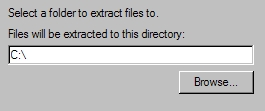
\includegraphics[width=0.35\linewidth]{images/avrgcc_0a}
				\caption{Ekstrak ke C:\textbackslash}
			\end{figure}
			
			\item Masukkan alamat kompiler dalam \textit{binary path} milik Windows.
			Buka System Variables. Klik Kanan \textbf{My Computer} -> \textbf{Properties} -> tab \textbf{Advanced} -> \textbf{Environment Variabels}.
			Klik dua kali variabel \textbf{Path} pada \textbf{System Variables}

			\begin{figure}[H]
				\centering
				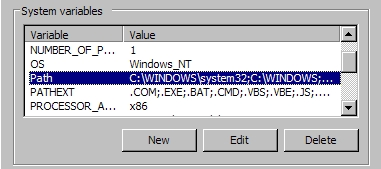
\includegraphics[width=0.35\linewidth]{images/avrgcc_0b}
				\caption{System Variables PATH}
			\end{figure}
			
			\item Kemudian masukkan alamat folder \textbf{bin} dari compiler, sebagai contoh:\\
			\textbf{;C:\textbackslash avr-gcc-8.3.0-x86-mingw\textbackslash bin}.
			Jangan lupa tanda titik-koma (;) diawal alamat sebagai pemisah.
			\begin{figure}[H]
				\centering
				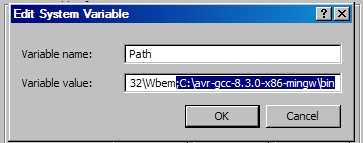
\includegraphics[width=0.35\linewidth]{images/avrgcc_0c}
				\caption{System Variables PATH}
			\end{figure}
		
			\item Selanjutnya Buka Code::Blocks. Klik menu \textbf{Settings} -> \textbf{Compiler}.\\
			Pilih compiler \textbf{GNU GCC Compiler for AVR}.\\
			Pilih Tab \textbf{Toolchain Executables} dan klik \textbf{Auto-detect}.

			\begin{figure}[H]
				\centering
				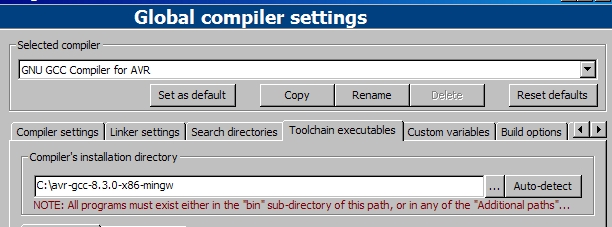
\includegraphics[width=0.75\linewidth]{images/avrgcc_0d}
				\caption{System Variables PATH}
			\end{figure}
			
		\end{itemize}
		
		\item Ubuntu/Debian.
		\begin{itemize}
			\item Buka Terminal (pastikan terhubung internet).
			\item Masukkan perintah.
			\begin{minted}[frame=lines,fontsize=\footnotesize]{bash}
sudo apt-get install gcc-avr binutils-avr avr-libc
			\end{minted}
			\item Tunggu proses selesai.
		\end{itemize}
		
		\item Fedora.
		\begin{itemize}
			\item Buka Terminal (pastikan terhubung internet).
			\item Masukkan perintah.
			\begin{minted}[frame=lines,fontsize=\footnotesize]{bash}
sudo dnf install avr-binutils avr-gcc avr-libc
			\end{minted}
			\item Tunggu proses selesai.
		\end{itemize}
		
		\item Arch-Linux.
		\begin{itemize}
			\item Buka Terminal (pastikan terhubung internet).
			\item Masukkan perintah.
			\begin{minted}[frame=lines,fontsize=\footnotesize]{bash}
sudo pacman -S avr-binutils avr-gcc avr-lib 
			\end{minted}
			\item Tunggu proses selesai.
		\end{itemize}
		
	\end{itemize}

	\newpage
	\subsubsection{Simul-IDE}
	
	Dalam kursus ini, untuk awal pelatihan, digunakan Simulator untuk menjalankan dan menguji program AVR yang dibuat.
	Simulator yang dipilih disini adalah Simul-IDE. 
	Simul-IDE adalah simulator rangkaian elektronik Digital/Analog sederhana yang dapat berjalan secara \textit{real-time}.
	Simul-IDE dapat mendukung microcontroller seperti chip seri AVR ataupun PIC.
	
	\begin{figure}[H]
		\centering
		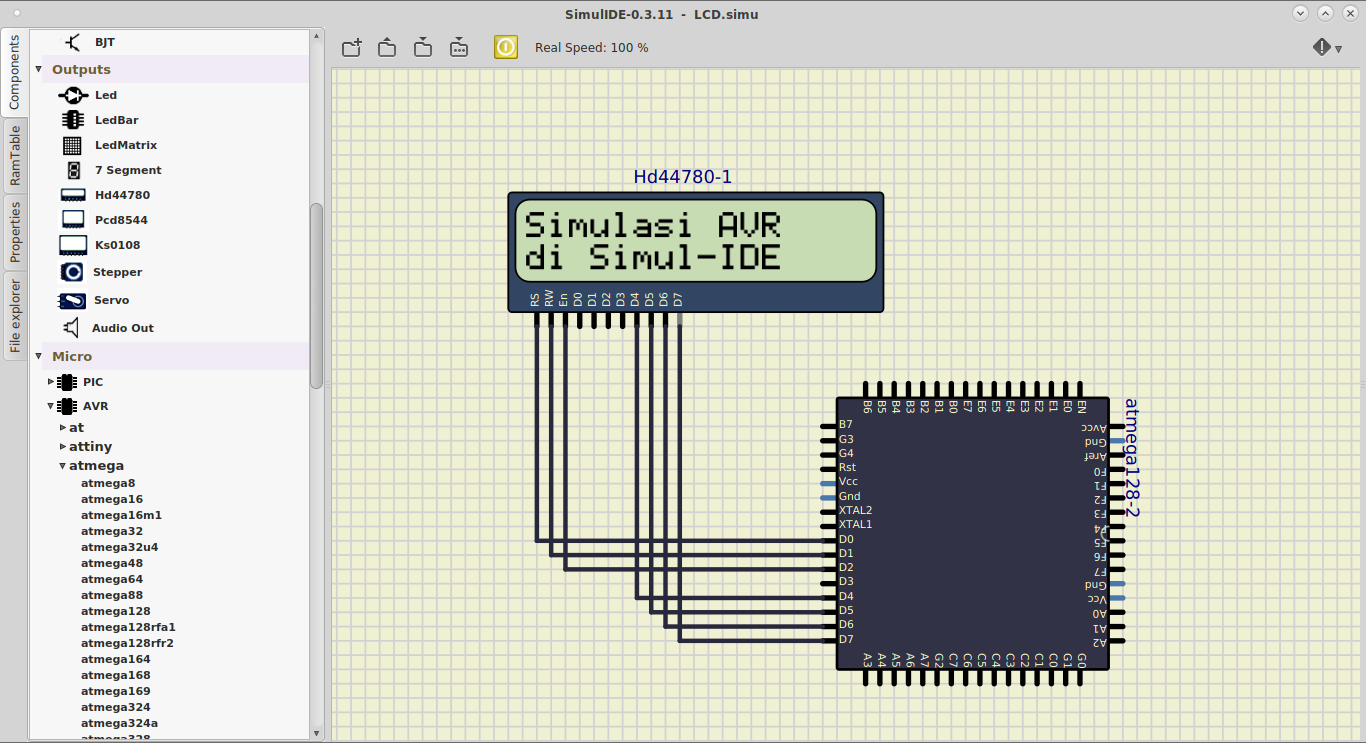
\includegraphics[width=0.6\linewidth]{images/simul}
		\caption{contoh tampilan Simul-IDE}
	\end{figure}
	
	Berikut untuk instalasi:
	\begin{itemize}
		\item Windows
		\begin{itemize}
			\item Buka alamat Simul-IDE:\\
			\url{https://sourceforge.net/projects/simulide/files/SimulIDE_0.3.10/SimulIDE_0.3.10_SR1-Win32.zip/download}
			
			\item Extrak file zip yang sudah di download ke C:\textbackslash.
			\begin{figure}[H]
				\centering
				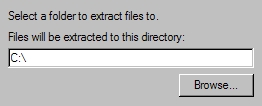
\includegraphics[width=0.35\linewidth]{images/simulide_0a}
				\caption{Ekstrak ke C:\textbackslash}
			\end{figure}
		
			\item Setelah selesai ekstraksi, buka forlder bin di alamat hasil ekstraksi.
			Contoh disini adalah alamat \textbf{C:\textbackslash SimulIDE\_0.3.10\_SR1-Win32\textbackslash bin}.

			\begin{figure}[H]
				\centering
				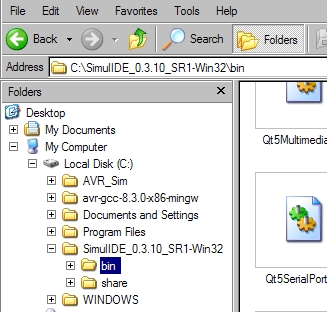
\includegraphics[width=0.35\linewidth]{images/simulide_0b}
				\caption{buka folder bin}
			\end{figure}
	
			\newpage
			\item Klik dua kali file \textbf{simulide.exe}.
			\begin{figure}[H]
				\centering
				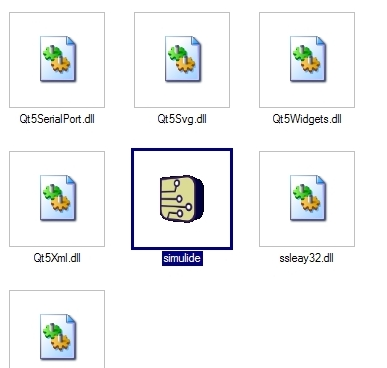
\includegraphics[width=0.35\linewidth]{images/simulide_0c}
				\caption{jalankan simulide.exe}
			\end{figure}
		
		\end{itemize}
		
		\item Ubuntu/Debian.
		\begin{itemize}
			\item Buka Terminal (pastikan terhubung internet).
			\item Masukkan perintah.
			\begin{minted}[frame=lines,fontsize=\footnotesize]{bash}
sudo apt-get install simulide simavr
			\end{minted}
			\item Tunggu proses selesai.
			\item Buka terminal dimana project AVR berada.
			\item Masukkan perintah:
			\begin{minted}[frame=lines,fontsize=\footnotesize]{bash}
simulide
			\end{minted}
		\end{itemize}
		
		\item Fedora.
		\begin{itemize}
			\item Buka Terminal (pastikan terhubung internet).
			\item Masukkan perintah.
			\begin{minted}[frame=lines,fontsize=\footnotesize]{bash}
sudo dnf install simulide simavr
			\end{minted}
			\item Tunggu proses selesai.
			\item Buka terminal dimana project AVR berada.
			\item Masukkan perintah:
			\begin{minted}[frame=lines,fontsize=\footnotesize]{bash}
simulide
			\end{minted}
		\end{itemize}
		
		\item Arch Linux.
		\begin{itemize}
			\item Buka Terminal (pastikan terhubung internet).
			\item Masukkan perintah.
			\begin{minted}[frame=lines,fontsize=\footnotesize]{bash}
sudo pacman -S simavr
			\end{minted}
			\item Tunggu proses selesai.
			\item Download resep AUR di \url{https://aur.archlinux.org/cgit/aur.git/snapshot/simulide.tar.gz}
			\item Ekstrak file tersebut dan buka terminal di alamat tersebut.
			\item Masukkan perintah:
			\begin{minted}[frame=lines,fontsize=\footnotesize]{bash}
makepkg -sir
			\end{minted}
			\item Tunggu proses instalasi selesai
			\item Buka terminal dimana project AVR berada.
			\item Masukkan perintah:
			\begin{minted}[frame=lines,fontsize=\footnotesize]{bash}
simulide
			\end{minted}
		\end{itemize}
		
	\end{itemize}

	\newpage
	\subsection{Hello World}
	
	Berikut akan didemonstrasikan bentuk paling sederhana (Hello World) untuk aplikasi ATMega.
	
	Contoh ini dibagi dalam bagian, yaitu membuat program dengan Code:Blocks dan simulasi dengan Simul-IDE.
	Semua contoh ini menggunakan ATMega-16.
	
	\subsubsection{Pemrograman: Project}
	
	Ikuti langkah-langkah berikut:
	\begin{itemize}
		\item Buat folder di C:\textbackslash, D:\textbackslash, atau dimana saja yang di alamat nya tidak memiliki spasi.
		Contoh disini di \textbf{C:\textbackslash AVR\_Sim\textbackslash}.
		
		\item Salin file \textbf{Makefile} ke folder tersebut.
		Makefile adalah file teks yang menjadi resep untuk kompilasi file source/header menjadi binary ELF/HEX/BIN.
		File Makefile dapat anda minta ke penulis atau download di alamat \href{https://minhaskamal.github.io/DownGit/#/home?url=https://github.com/mekatronik-achmadi/my_examples/blob/master/atmega/ATMegaBasic/ALCD/Makefile}{disini}.
		
		\begin{figure}[H]
			\centering
			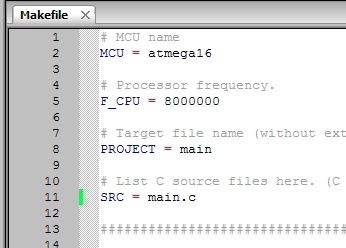
\includegraphics[width=0.5\linewidth]{images/hello_a0}
			\caption{potongan Makefile}
		\end{figure}
	
		\item Buat project baru.
		\begin{figure}[H]
			\centering
			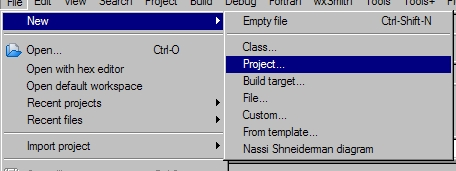
\includegraphics[width=0.5\linewidth]{images/hello_a1}
			\caption{project baru}
		\end{figure}
	
		\newpage
		\item Pilih \textbf{Empty Project}.
		\begin{figure}[H]
			\centering
			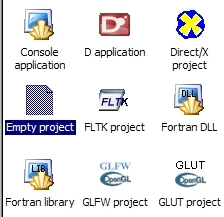
\includegraphics[width=0.4\linewidth]{images/hello_a2}
			\caption{project kosong}
		\end{figure}
	
		\item Isi nama project sama dengan nama folder project.
		Alamat project adalah satu level di atas.
		Sehingga project Code::Blocks satu folder dengan Makefile.
		\begin{figure}[H]
			\centering
			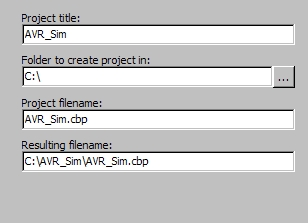
\includegraphics[width=0.5\linewidth]{images/hello_a3}
			\caption{isi nama project}
		\end{figure}
		
		\newpage
		\item Pilih compiler \textbf{GNU GCC Compiler for AVR}.
		Bersihkan centang \textbf{Debug}.
		Isi target release dengan \textbf{all}.
		Bersihkan semua dir.
		\begin{figure}[H]
			\centering
			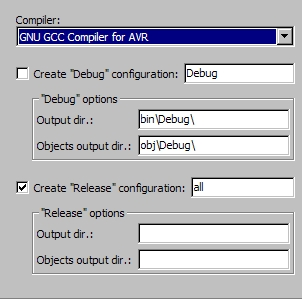
\includegraphics[width=0.5\linewidth]{images/hello_a4}
			\caption{Pilih compiler}
		\end{figure}
	
		\item Setelah project baru selesai dibuat, klik menu \textbf{Project} -> \textbf{Properties}.
		Pilih tab \textbf{Project Settings}.
		Centang opsi \textbf{This is a custom Makefile}.
		\begin{figure}[H]
			\centering
			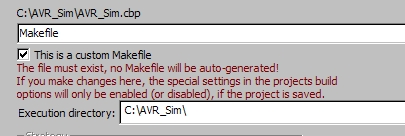
\includegraphics[width=0.5\linewidth]{images/hello_a5}
			\caption{custom Makefile}
		\end{figure}
		
		\item Selanjutnya atur perintah untuk clean, klik menu \textbf{Project} -> \textbf{Build Option}.
		Pilih tab \textbf{"Make" commands}.
		Pada kolom Clean Project/target, hapus kata '\$target' dibelakang 'clean'
		\begin{figure}[H]
			\centering
			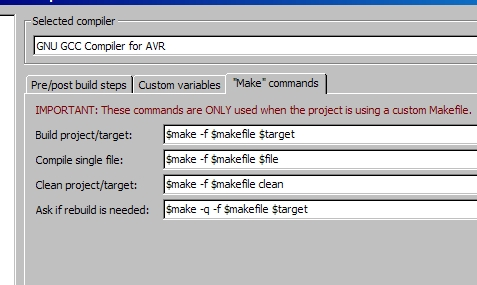
\includegraphics[width=0.5\linewidth]{images/hello_a6}
			\caption{target clean}
		\end{figure}
	
		\item Selanjutnya tambahkan Makefile ke Project.
		Klik kanan project, pilih \textbf{Add files}.
		\begin{figure}[H]
			\centering
			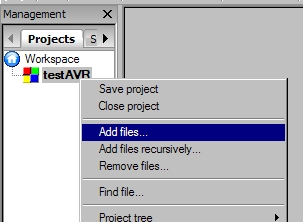
\includegraphics[width=0.5\linewidth]{images/hello_a7}
			\caption{tambah file yang sudah ada}
		\end{figure}
	
		\item Pilih Makefile di folder project.
		Klik kanan project, pilih \textbf{Add files}.
		\begin{figure}[H]
			\centering
			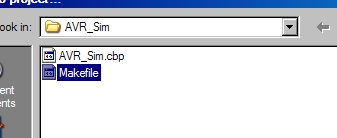
\includegraphics[width=0.5\linewidth]{images/hello_a8}
			\caption{tambah Makefile}
		\end{figure}
		
		\item Demikian minimum project yang perlu dibuat.
	\end{itemize}
	
	\subsubsection{Pemrograman: Sources}
	
	Selanjutnya file untuk C sources nya.
	Berikut langkahnya.
	\begin{itemize}
		\item Buat file baru.
		\begin{figure}[H]
			\centering
			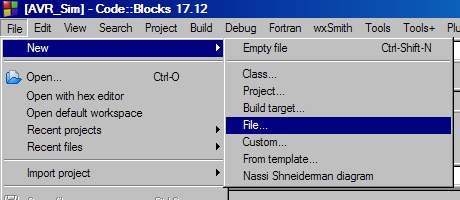
\includegraphics[width=0.5\linewidth]{images/hello_a9}
			\caption{tambah file baru}
		\end{figure}
	
		\newpage
		\item Pilih C/C++ Sources
		\begin{figure}[H]
			\centering
			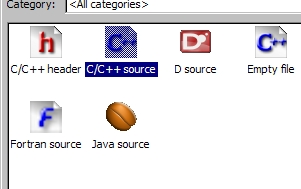
\includegraphics[width=0.5\linewidth]{images/hello_a10}
			\caption{pilih C/C++}
		\end{figure}
	
		\item Pilih C
		\begin{figure}[H]
			\centering
			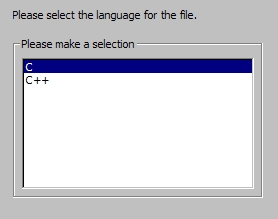
\includegraphics[width=0.5\linewidth]{images/hello_a11}
			\caption{pilih C}
		\end{figure}
	
		\item Pilih isi nama file.
		Disini dicontohkan \textbf{main.c}.
		\begin{figure}[H]
			\centering
			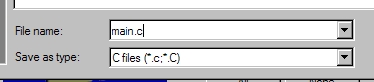
\includegraphics[width=0.5\linewidth]{images/hello_a12}
			\caption{main.c}
		\end{figure}
	
		\newpage
		\item pastikan \textbf{add file to active project} dan \textbf{all} dicentang.
		Disini dicontohkan \textbf{main.c}.
		\begin{figure}[H]
			\centering
			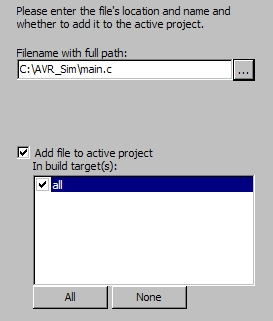
\includegraphics[width=0.5\linewidth]{images/hello_a13}
			\caption{selesai main C}
		\end{figure}
		
		\item bila diperlukan, cek file masuk ke active project.
		\item Setelah project baru selesai dibuat, klik menu \textbf{Project} -> \textbf{Properties}.
		Pilih tab \textbf{Build targets}.
		Lihat kolom terbawah (\textbf{Build Target files}).
		Pastikan semua tercentang.
		\begin{figure}[H]
			\centering
			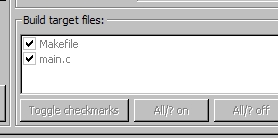
\includegraphics[width=0.5\linewidth]{images/hello_a14}
			\caption{selesai main C}
		\end{figure}
		
	\end{itemize}

	\newpage
	\subsubsection{Pemrograman: Building}
	
	Berikut isi untuk \textbf{main.c}
	\begin{minted}[frame=lines,fontsize=\footnotesize]{c}
#include <avr/io.h>
#include <utils/delay.h>

int main(void){
	DDRC |= 1<<0;
	
	while(1){
		PORTC |= 1<<0;
		_delay_ms(200);
		
		PORTC &= ~(1<<0);
		_delay_ms(200);
	}
	
	return 0;
}
	\end{minted}
	
	Selanjutnya untuk isi \textbf{Makefile}, untuk saat tidak perlu diperhatikan semua, cukup 4 parameter teratas.
	Yaitu:
	\begin{itemize}
		\item \textbf{MCU}. Disini didefinisikan jenis chip avr yang akan digunakan.
		Daftar MCU yang dapat digunakan bisa dilihat di alamat:\\
		\url{https://gcc.gnu.org/onlinedocs/gcc-4.8.5/gcc/AVR-Options.html}.
		
		\begin{minted}[frame=lines,fontsize=\footnotesize]{bash}
MCU = atmega16
		\end{minted}
		
		\item \textbf{F\_CPU}. Disini didefinisikan nilai clock dalam satuan Hz.
		Untuk hardware asli, didapat dari nilai crystal, internal rtc, dst sesuai pengaturan fuse bit.
		Untuk simulasi, bisa dilihat di \textit{properties} objek simulasi.
		Nilai yang umum adalah 8MHz,11.0592MHz, 12MHz, dan 16 MHz.
		\begin{minted}[frame=lines,fontsize=\footnotesize]{bash}
F_CPU = 8000000
		\end{minted}
		
		\item \textbf{PROJECT}. Disini didefinisikan nama akhir binary nanti.
		Nama bebas, asal jangan terlalu panjang, tidak diawali angka, tanpa spasi, simbol matematis, namun underscore diperbolehkan.
		\begin{minted}[frame=lines,fontsize=\footnotesize]{bash}
PROJECT = main
		\end{minted}
		
		\item \textbf{SRC}. Disini didaftarkan file C yang akan di kompilasi.
		File C bisa lebih dari satu dan dipisah oleh spasi.
		\begin{minted}[frame=lines,fontsize=\footnotesize]{bash}
SRC = main.c
		\end{minted}
	\end{itemize}

	Jika semua sudah disiapkan, klik menu \textbf{Build}->\textbf{Build}.
	Jika tidak ada kesalahan, maka hasil akhir binary ELF (*.elf), HEX (*.hex), dan BIN (*.bin) akan muncul.
	
	\subsubsection{Simulasi}
	
	Selanjutnya, dilakukan demonstrasi menggunakan Simul-IDE.
	Berikut langkah-langkahnya.
	\begin{itemize}
		\item Jalankan program Simul-IDE dengan klik dua kali simulide.exe
		
		\item Masukkan komponen yang dibutuhkan.
		Caranya adalah "menarik" komponen ke kanvas.
		Berikut komponen yang dibutuhkan.
		\begin{enumerate}
			\item ATMega16. [Micro -> AVR -> atmega].
			\item LED. [Outputs].
			\item Ground 0v. [Sources].
		\end{enumerate}
	
		\begin{figure}[H]
			\centering
			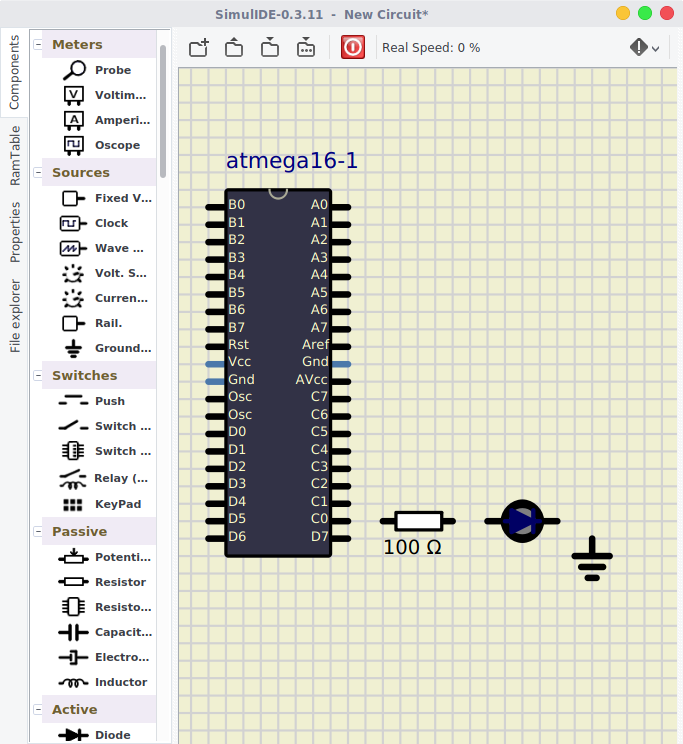
\includegraphics[width=0.5\linewidth]{images/tessim_0}
			\caption{komponen}
		\end{figure}
	
		\item Wiring komponen.
		Caranya adalah klik kaki yang kosong, drag kabel ke kaki tujuan.
		Sambungan yang dibutuhkan:
		\begin{enumerate}
			\item pin C0 ke anoda LED.
			\item pin katoda LED ke GND
		\end{enumerate}
	
		\begin{figure}[H]
			\centering
			\includegraphics[width=0.5\linewidth]{images/tessim_1}
			\caption{circuit}
		\end{figure}
	
		\item masukkan file *.elf atau *.hex yang akan disimulasikan.
		Klik kanan ATMega 16, pilih menu \textbf{Load firmware}.
		
		\begin{figure}[H]
			\centering
			\includegraphics[width=0.5\linewidth]{images/tessim_2}
			\caption{load firmware}
		\end{figure}
		
		dan cari file *.elf atau *.hex yang akan disimulasikan.
		
		\begin{figure}[H]
			\centering
			\includegraphics[width=0.5\linewidth]{images/tessim_3}
			\caption{pilih file binary}
		\end{figure}
		
		\item Selanjutnya, tekan tombol merah untuk menjalankan simulasi.
		Tombol kuning berarti simulasi sedang berjalan. Tekan untuk menghentikan.
		
		\begin{figure}[H]
			\centering
			\includegraphics[width=0.25\linewidth]{images/tessim_off}
			\caption{simulation off}
			\includegraphics[width=0.25\linewidth]{images/tessim_on}
			\caption{simulation on}
		\end{figure}
	
		\item Pada Tahap Ini, seharusnya LED akan berkelip.
		
		\begin{figure}[H]
			\centering
			\includegraphics[width=0.5\linewidth]{images/tessim_4}
			\caption{LED berkelip}
		\end{figure}
		
		\item Jika program dimodifikasi, maka untuk memasukkan ulang program tidak perlu pilih \textbf{Load firmware},
		melainkan menu \textbf{Reload firmware}.
		
		\begin{figure}[H]
			\centering
			\includegraphics[width=0.5\linewidth]{images/tessim_5}
			\caption{reload firmware}
		\end{figure}
	\end{itemize}
	
\end{document}
